\documentclass[11pt,a4paper,uplatex]{ujreport} 	% for uplatex
%
\usepackage{amsmath,amssymb}
\usepackage{bm}
\usepackage{graphicx}
\usepackage{ascmac}
\usepackage{float}
%
\setlength{\textheight}{40\baselineskip}
\addtolength{\textheight}{\topskip}
\setlength{\voffset}{-0.2in}
\setlength{\topmargin}{0pt}
\setlength{\headheight}{0pt}
\setlength{\headsep}{0pt}

\setlength{\textwidth}{\paperwidth}     % ひとまず紙面を本文領域に
\setlength{\oddsidemargin}{-5.4truemm}  % 左の余白を20mm(=1inch-5.4mm)に
\setlength{\evensidemargin}{-5.4truemm} % 
\addtolength{\textwidth}{-40truemm}     % 右の余白も20mmに
%

\newcommand{\argmax}{\mathop{\rm arg~max}\limits}
\newcommand{\argmin}{\mathop{\rm arg~min}\limits}


\title{脳波解析のための数学シリーズ\\
統計編}
\author{後藤 優仁}
\date{\today}
\begin{document}
\maketitle

\newpage
%
%
\tableofcontents
\newpage
\chapter{はじめに}
 統計処理とは, 実際に実験やアンケートを通して集めたデータを解釈する際に必要になる処理です. 論文を読むためにも必須, というか一番大事な項目なので頑張りましょう. analysisの様々な処理を行った結果,実験で計測した脳波を何らかの形で解釈しやすいようなデータに変形する事が出来ました.つまり解析をしました.次に必要なのは,この解析で得られたデータを解釈する行程です.ここで必要になるのが統計的な処理ですね.個人的には楽しくないですが,仕方ないのでやっていきましょう.\\
  また,結局脳の計算をモデル化しようとか発展的な議論をしていこうと思った時にはここら辺が非常に重要になってきます.先に勉強しておくとだいぶ後が楽だと思いますが,何に役立つのか分からないとモチベは上がらないし勉強できないのは自分も痛いほど分かるので,逆に先にadvanced.pdfとかでチラ見してくるのも良いかもしれませんね.\\

あと検定.正味これがいっちゃん大事なのですがいっちゃん勉強する気になれないんですよねぇ...がんばります.
 
 \newpage
 
 
\chapter{確率分布}
基礎編に乗っているような基礎統計量だけの議論では必要ないため,(多分)高校数学ではやりませんが,それ以上の統計学をやる上で必須になってくるのが確率分布の概念です.\\
\\

世の中には無数の統計的データがある,というか収集できますが,そいつらの統計的な分布,つまりヒストグラムの形は概ねいくつかの典型的なパターンのどれかに当てはまる事が知られています.中でも正規分布という分布はつよつよで,中心極限定理という定理が示すように世の中の多くの事象に適用できる分布の形です.\\

こいつらを知っている事で,その性質から考えて,実際に得られたデータの平均や分散といった値はどうなのか(推定),そもそも普通にありえる話なのか,何か特殊な事情で一般的ではないデータが取られたのか(統計的検定)や,では次に来る事象はどうなる可能性が高いか(予測)など様々な議論を展開していく事が可能になります.\\

そのため,確率分布はそれだけで学んだところで特に面白味がありませんが,今後使っていくという意味では重要です.ここでは,代表的な確率分布を載せていきます.覚える必要はないので,どんな奴らがいるのかなんとなく見て,3章以降で出てきた際に参照できるようにしておきましょう.
\section{確率分布と確率密度関数}
まずは定義の確認から改めて行っておきましょう!\\

確率とは, 起こりうる全体の事象のうち, ある事象がどれくらいの割合で起こるのかを表します. \\

確率分布とは, 起こりうる事象それぞれの確率がどのような分布をしているかです. \\

確率密度関数とは, 実際に確率分布をプロット(横軸に事象, 縦軸に確率)した際に現れる分布の形を表現する関数の事です. 場合によっては事象は離散分布になったりするため,その場合はこの分布を連続と見立てて確率密度関数が定義されます.\\

\section{一様分布/ベルヌーイ分布/2項分布/ポアソン分布}
まずは簡単な分布から見て, 徐々に複雑なものを見ていきます. 今回は脳の数学であまり使わない気がするやつらはまとめて雑に確認します.\\
\subsection{一様分布}
例えばサイコロを振った時に出る目の確立分布を考えると, 当然6つの事象それぞれがすべて$\frac{1}{6}$で表せるため, プロットすると以下のようになります.\\
\begin{figure}[H]
\label{im:uniform}
  \centering
  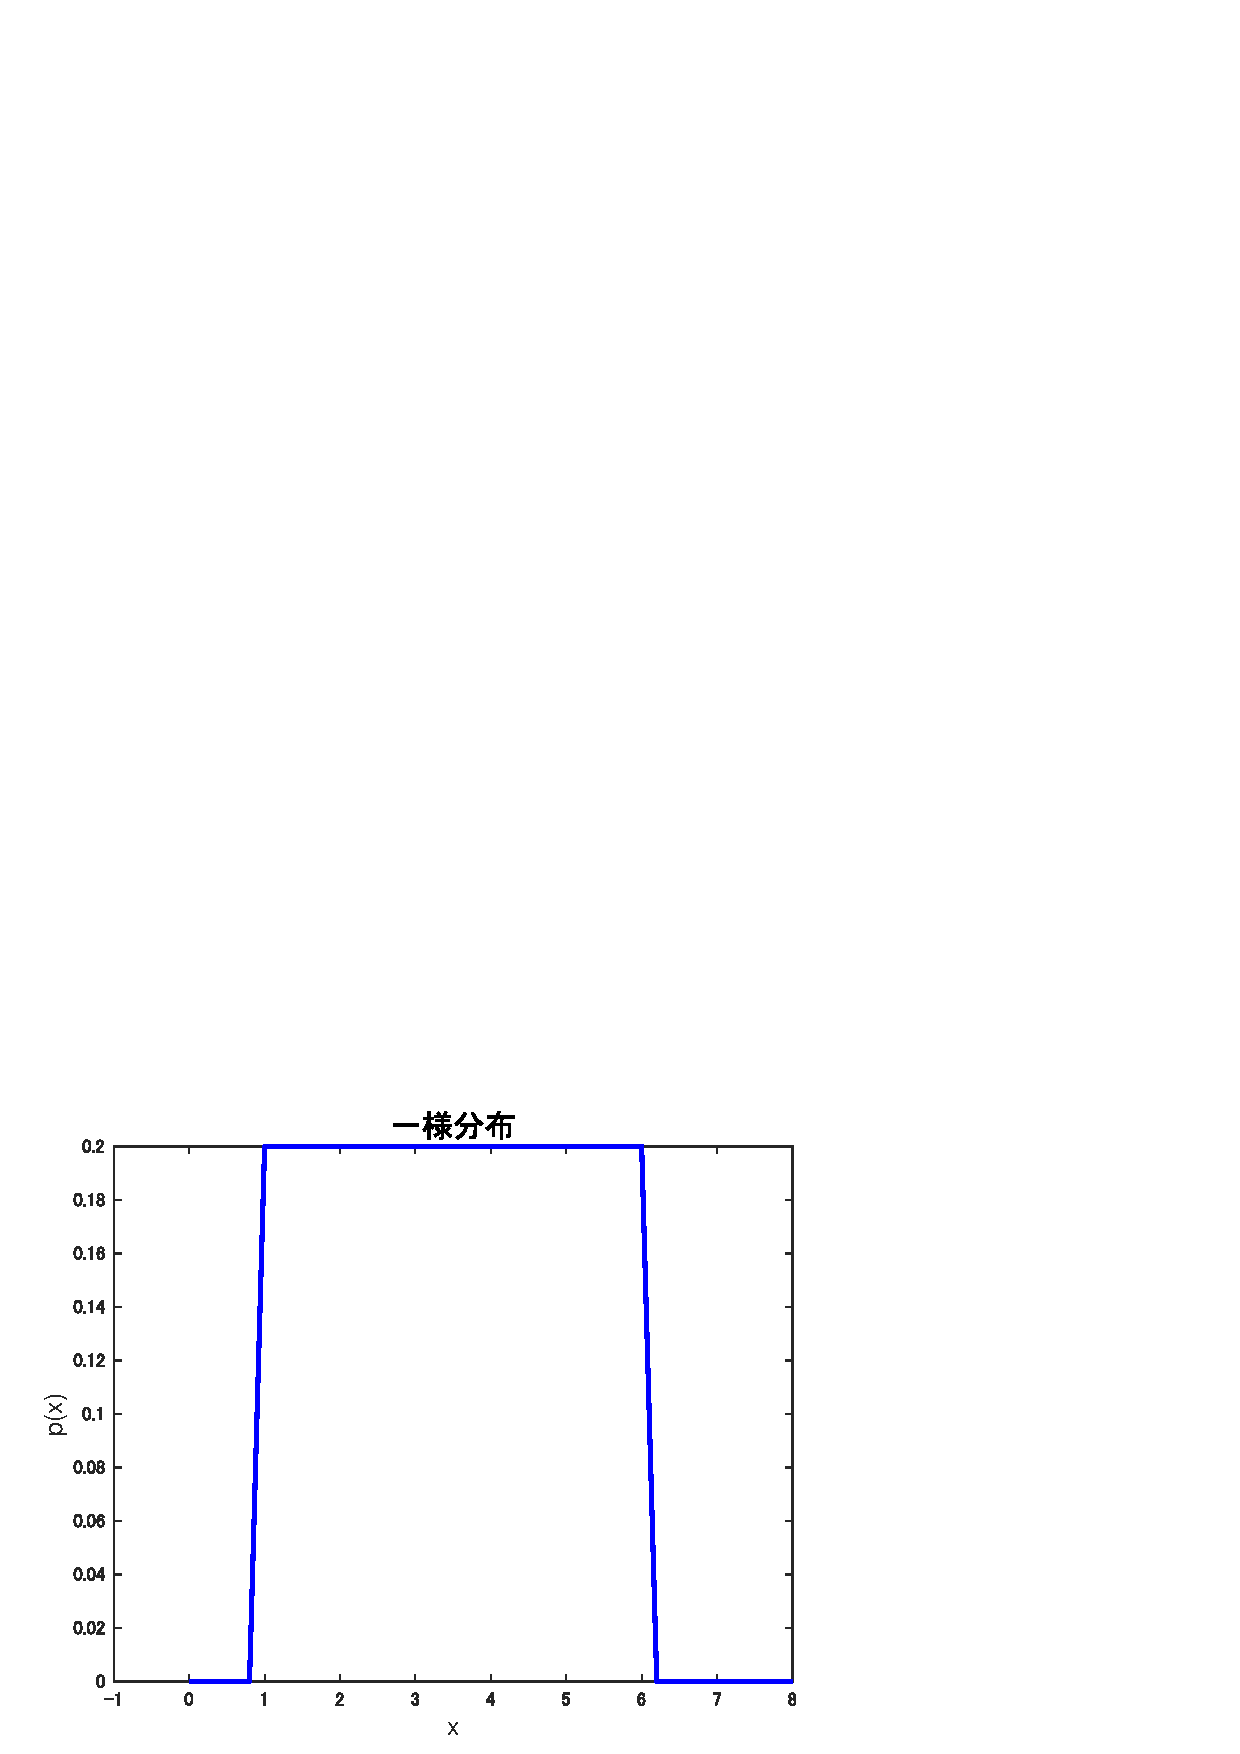
\includegraphics[width=120mm,bb=0 0 432 288]{../figures/uniform.png}
  \caption{サイコロの確立分布(一様分布)}
\end{figure}

一様分布は確率密度関数を定義するまでもないのですが, 勉強のためにあえてやるとすると以下のようになります. まずさいころの例だとそれぞれの目が出てくる確率はこうですね.

\begin{align}
\label{eq:uniform}
f(x) = \frac{1}{6} (1 \leq X \leq 6)
\end{align}

定義域が0から6で, いずれの点においても$\frac{1}{6}$の確立で目がでるよってことですね. 簡単です. また確率を考える際, 式(\ref{eq:uniform})のように左辺の$(x)$と右辺定義域内にいる$(X)$で使い分けがなされます. $X$は確率変数を表し, 実際の値は取りません. 観測されて確定した時には$x$として表現されます. 今回の$X$と$x$の関係は

\begin{align}
X = [x_1, x_2, x_3, x_4, x_5, x_6]
\end{align}

のような感じです. \\
\\

より一般には離散一様分布に従う変数の確率関数は,Nを変数が取りうる値(さいころの目=6)として,

\begin{align}
P(X=x) = \frac{1}{N} \qquad (x=1,2,...,N)
\end{align}

となります.これはさすがに良いですよね.次.\\

離散一様分布の期待値と分散は以下です.\\

\begin{align}
\mathbb{E}(X) &= \sum_{k=1}^N{kP(X=k)}\\
&=\sum_{k=1}^N{k\frac{1}{N}}\\
&= \frac{(1+N)N}{2}\frac{1}{N}\\
&= \frac{1+N}{2}
\end{align}

\begin{align}
\mathbb{V}(X) &= \mathbb{E}(X^2) - \mathbb{E}(X)^2\\
&= \sum_{k=1}^N k^2 \frac{1}{N} - {(\frac{1+N}{2})}^2\\
&= \frac{1}{N}N\frac{(N+1)(2N+1)}{6}-\frac{(N+1)^2}{4}\\
&= \frac{N^2-1}{12}
\end{align}

一見複雑?な気もするかもしれませんが,普通に計算してみればわかるとおもいます.ほら,「1から100までの数の和は?」みたいな問題って工夫して暗算出来ましたよね?どうやるんでしたっけ.\\
\\

連続一様分布については確率密度関数は以下のようになります.

\begin{align}
f(x) = 
\left\{
    \begin{array}{l}
      \frac{1}{b-a} \qquad \qquad  (a \leq X \leq b) \\
      0  \qquad \qquad \qquad(otherwise)
    \end{array}
  \right.
\end{align}

これは面積で考えると分かりやすいかも.確率密度関数は積分すると1にならないといけません.b-aは定義域なので,つまり面積でいうところの横の長さです.縦の長さはそれぞれの値が観測される確率,つまり$f(x)$ですよね?\\

そう,なので定義の$f(x)$を定義域で積分すると1になります.当たり前の事なのですが,確率密度関数の考え方にいまいち慣れていない人ように丁寧に言いました.以下はこのような話は省略します.\\

とにかく,積分すると1になるのが確率密度関数です.


平均$\mathbb{E}(X)$及び分散$\mathbb{V}(X)$は

\begin{align}
\mathbb{E}(X) = \frac{a+b}{2}\\
\mathbb{V}(X) = \frac{(b-a)^2}{12}
\end{align}

一応,期待値くらいは証明もしておきます.でもまあ簡単です.

\begin{align}
\mathbb{E}(X)  &= \int_{-\infty}^{\infty} xf(x) dx \\
&= \int_{-\infty}^{a} xf(x) dx + \int_{a}^{b} xf(x) dx + \int_{b}^{\infty} xf(x) dx \\
&= 0 + \int_{a}^{b} x\frac{1}{b-a} dx + 0\\
&= \frac{1}{b-a}\left[\frac{x^2}{2}\right]_a^b\\
& = \frac{b-a}{2}
\end{align}

\subsection{ベルヌーイ分布}
ベルヌーイ分布は, 1か0かです. ある事が起きるか起きないか, 成功するかしないかなどの2値分類ですね. 超簡単です!!\\

\begin{figure}[H]
\label{im:bernoulli}
  \centering
  \includegraphics[width=120mm,bb=0 0 432 288]{../figures/bernoulli.png}
  \caption{ベルヌーイ分布}
\end{figure}

今回は1:1の図になっていますが, もちろん1:5くらいの割合になる事もあります. たとえばサイコロで1が出るか出ないかとか. 以上.\\
\\

関数はこんな感じかな
\begin{align}
f(x)=
  \left\{
    \begin{array}{l}
      p \qquad \qquad \qquad (x = 1) \\
      q(=1-p)  \qquad (x=0)
    \end{array}
  \right.
\end{align}

平均$\mathbb{E}(X)$及び分散$\mathbb{V}(X)$は

\begin{align}
\mathbb{E}(X) = p\\
\mathbb{V}(X) = pq
\end{align}

です. 興味ないので証明とかやりません. 僕も知らない.
\subsection{2項分布}
2項分布は「同じことを何回も繰り返した時, ある事柄が何回おこるか」の確立分布です. こいつは式を見れば早いですね.

\begin{align}
\label{eq:binomial}
f(x) = {}_n\mathrm{C}_x p^x(1-p)^{n-x}
\end{align}

式(\ref{eq:binomial})の右辺左側にある${}_n\mathrm{C}_x p^x$は, 確率pで起こる事象Aが, 全体nのうちx回でたという意味で, 右側の$(1-p)^{n-x}$は確率(1-p)で, Aが起きなかった回数が(n-x)回出たという意味です.\\

これらを掛け合わせているので, 何回当たって何回外れたかを表す式ですね.

\begin{figure}[H]
\label{im:bernoulli}
  \centering
  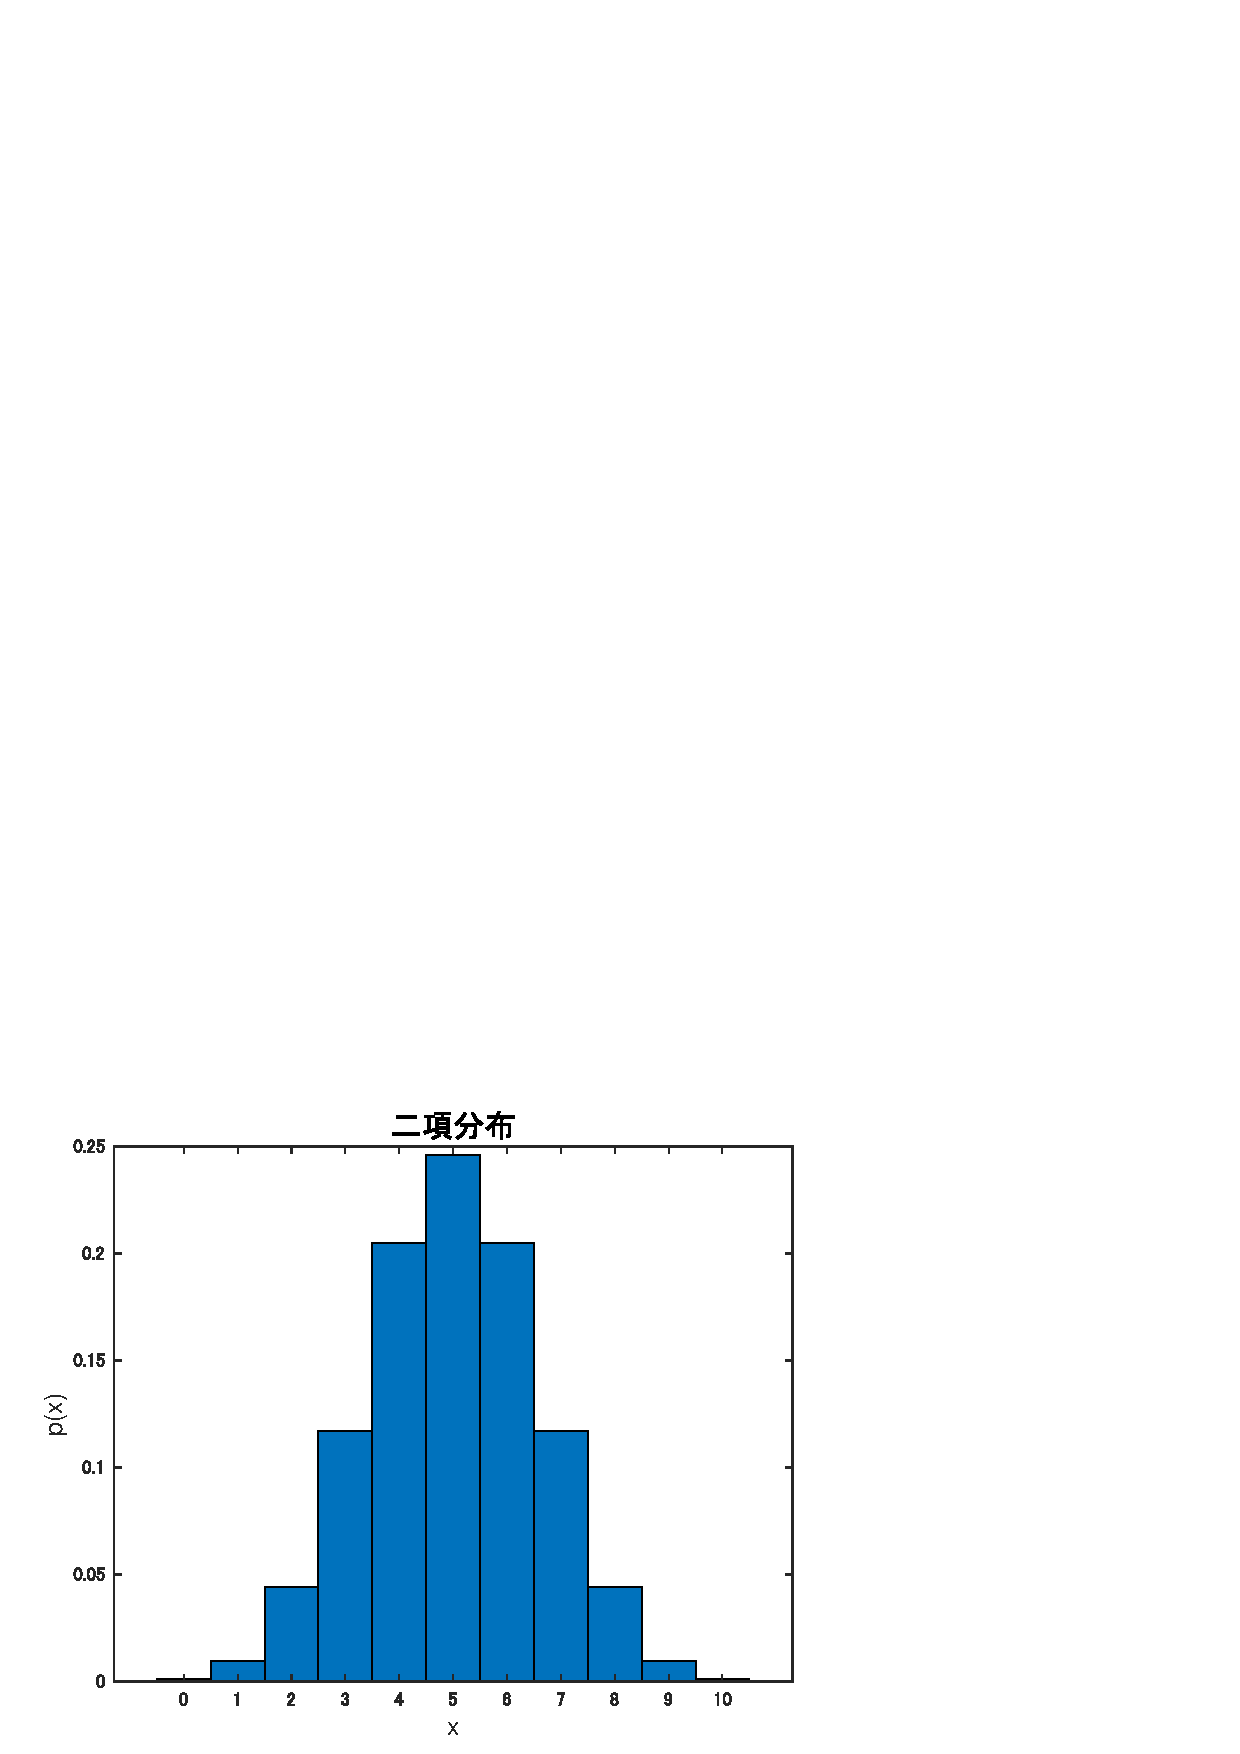
\includegraphics[width=120mm,bb=0 0 432 288]{../figures/binomial.png}
  \caption{ベルヌーイ分布}
\end{figure}

平均$\mathbb{E}(X)$及び分散$\mathbb{V}(X)$は

\begin{align}
\mathbb{E}(X) = np\\
\mathbb{V}(X) = np(1-p)
\end{align}

です. 興味ないので証明とかやりません. 僕も知らない.

\subsection{ポアソン分布}
ポアソン分布は「稀な事象が一定時間内にどれくらい起きるか」です.\\

たとえば, ある月にある地域で起きた交通死亡事故の件数とかです. 修羅の国やグンマ―, あるいは名古屋でもない限り, 普通は0か多くて2件とかですよね.\\
\\

確率密度関数は以下です.
\begin{align}
f(x) = \frac{\lambda^x}{x!}e^{-\lambda}
\end{align}

平均$\mathbb{E}(X)$及び分散$\mathbb{V}(X)$は

\begin{align}
\mathbb{E}(X) = \lambda\\
\mathbb{V}(X) = \lambda
\end{align}

です. こいつの場合, 平均も分散も同じ定数$\lambda$なので, こいつの値だけで形が決まります. $\lambda$がどんな値なのか, どうやって決まるのかは知りません. 使う事があれば足します.\\

\begin{figure}[H]
\label{im:poisson}
  \centering
  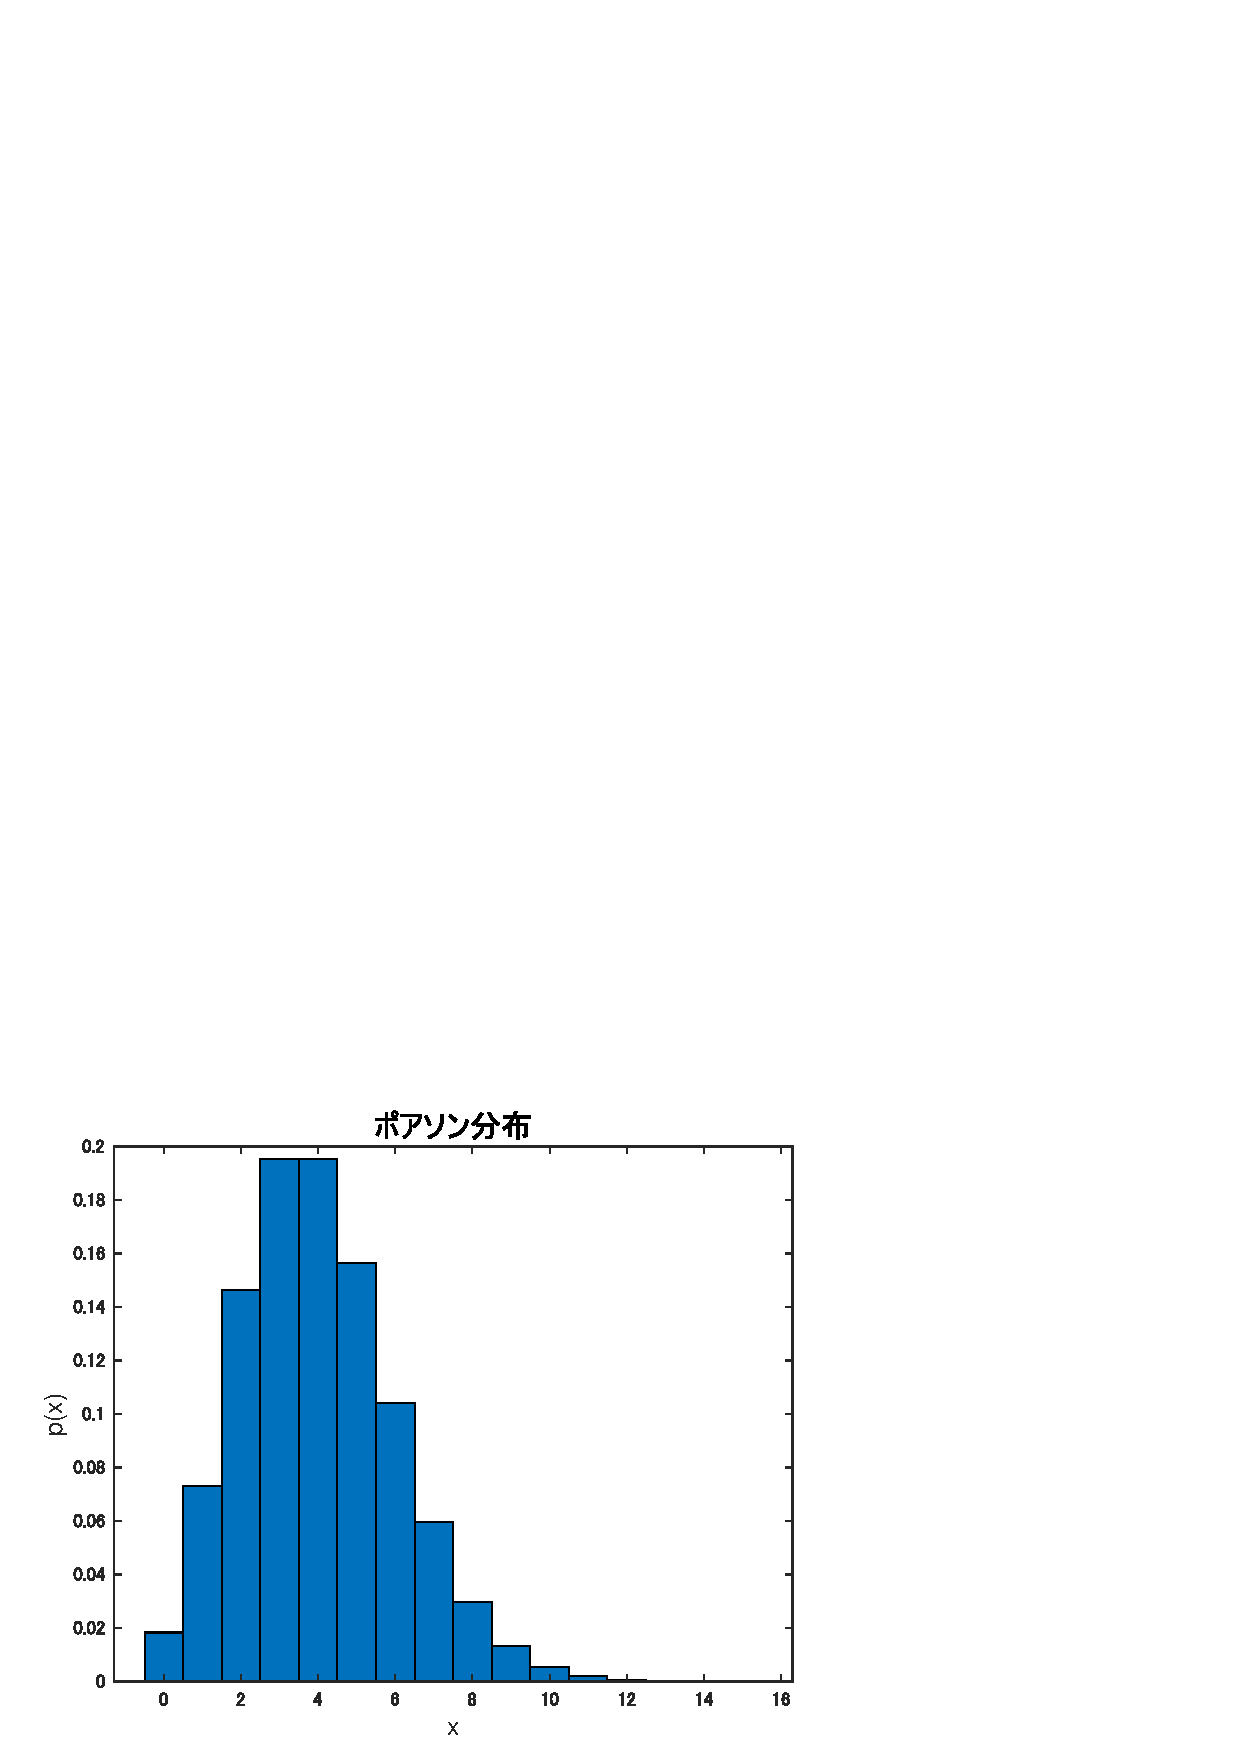
\includegraphics[width=120mm,bb=0 0 432 288]{../figures/poisson.png}
  \caption{ポアソン分布}
\end{figure}

\section{正規分布}
\subsection{正規分布とは}
さて本題です. 数ある確率分布の中でも抜きんでて重要な分布, 正規分布, またの名をガウス分布です. 世の中の多くの事象がこの分布に従っていて, また従っていると仮定して統計的処理がされています. 今後の統計学の基礎になるのでしっかり理解しましょう.\\
\\

正規分布は, 平均$\mathbb{E}(X)$が母集団の平均$μ$と等しく, 分散$\mathbb{V}(X)$も母集団の分散$\sigma ^2$と等しくなる分布で, 確率密度関数は以下になります.

\begin{align}
\label{eq:normal}
f(x) = \frac{1}{\sqrt{2\pi\sigma^2}}e^{-\frac{(x-\mu)^2}{2\sigma^2}}
\end{align}

いや, うん. 分かります. やばそうですよね. \\

ただまぁ, なんでこんな殺意高めな式になるのかは正規分布のグラフを見れば理解できます. 母集団の平均が50, 標準偏差20の正規分布だとこうなります.

\begin{figure}[H]
\label{im:normal}
  \centering
  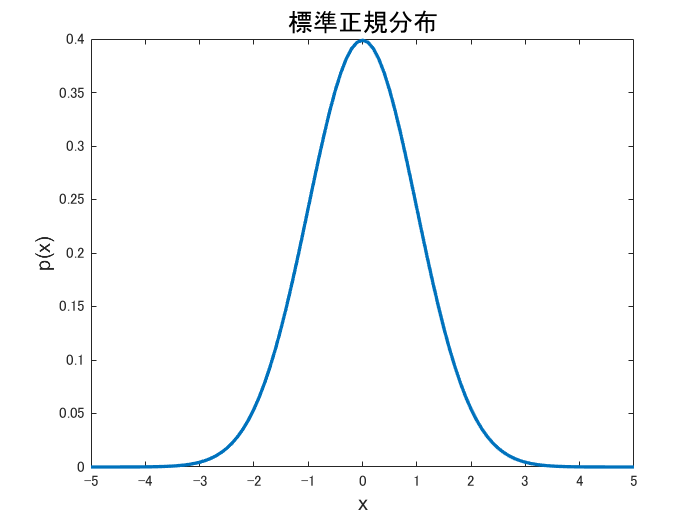
\includegraphics[width=120mm,bb=0 0 432 288]{../figures/normal.png}
  \caption{正規分布}
\end{figure}

定義通り, 確率変数の平均も50, 分散も400(20の二乗)になっていますね!!これが正規分布です. 綺麗ですね.\\
\\
\subsection{確率密度関数の導出}
さて, 式(\ref{eq:normal})の解説です. まずややこしいとこを全て消し飛ばし, 以下のように変形しましょう. 

\begin{align}
\label{eq:normal2}
f(x) = e^{-x^2}
\end{align}

\begin{figure}[H]
\label{im:normal}
  \centering
  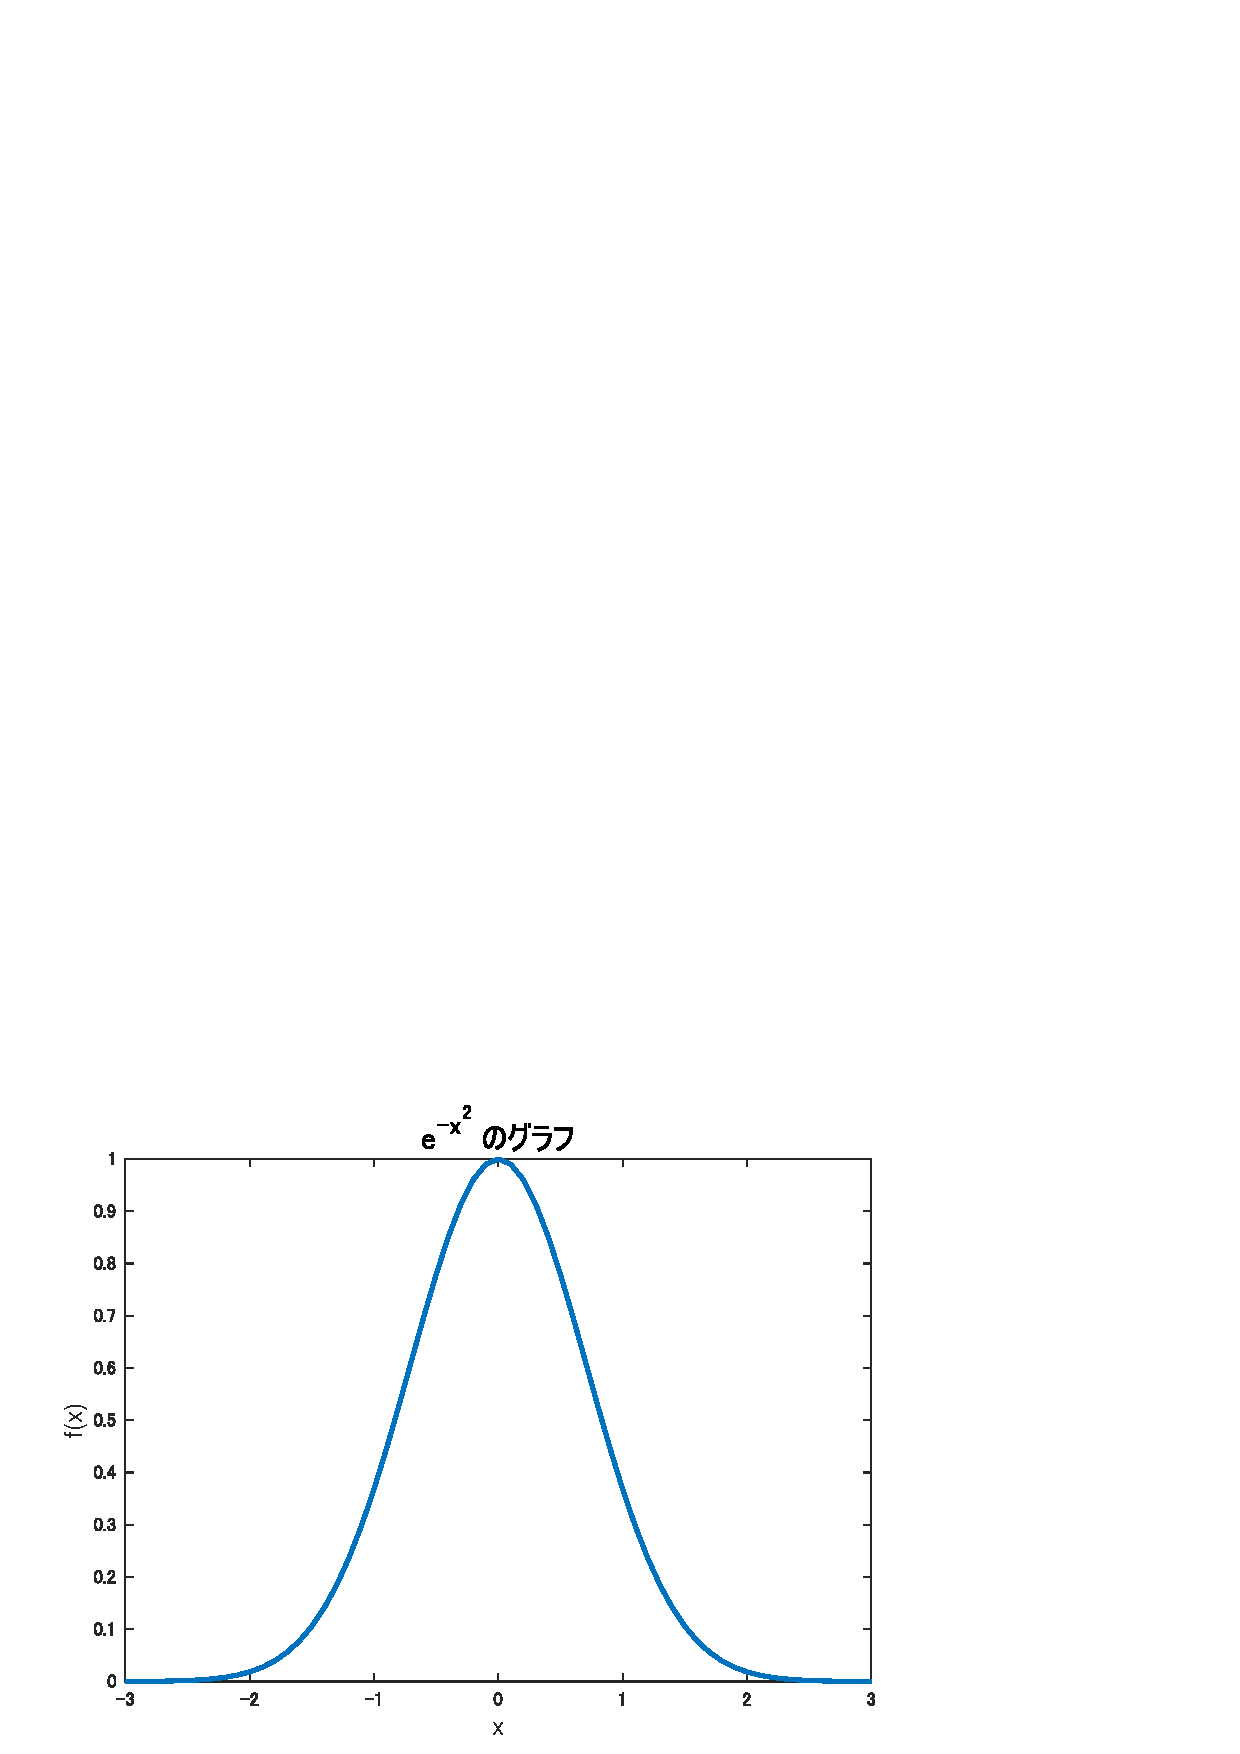
\includegraphics[width=120mm,bb=0 0 432 288]{../figures/normal2.png}
  \caption{式(\ref{eq:normal2})の図}
\end{figure}

この関数の説明はいりませんね? 指数関数の二乗の負版です.\\

まず, 世の中の多くの事象は平均値を取る確率が一番大きく, 平均値から離れるにつれその値を取る確率は小さくなることが知られています. んで, これをどう数式で表現すれば良いかと悩んだ末考えだされたのが正規分布関数だと思ってください.\\

そうすると, とりあえず釣り鐘型の関数が欲しいという事で式(\ref{eq:normal2})を考えました. 実際これでほぼ完成です.\\

ただ, これは任意定数がないため平均が0, 分散(幅)も一定ですね. これでは実用できません. そこで任意定数を導入し, 平均値と分散を可変にします. \\

まずは平均値, つまりこのグラフの頂点の位置を動かします.\\

\begin{align}
\label{eq:normal3}
f(x) = e^{-(x-\mu)^2}
\end{align}

二次関数で高校の時にやりましたね.\\

次に, 分散...つまりこの釣り鐘の幅というか広がり方を変えます. \\

\begin{align}
\label{eq:normal4}
f(x) = e^{-\frac{(x-\mu)^2}{\sigma^2}}
\end{align}

平均に比べて一寸難解かもしれません. σ, つまり標準偏差で割る事で, σの値が小さければ鋭く, 大きければ扁平なグラフになります.\\
\\
 ただ, σは正負が定まらないため, 二乗して分散の形にする事で符号を一定にするわけです. \\
\\
 ともあれ ... これで, 母平均と母分散によって形を変える釣り鐘型分布が完成です!!めでたい!!\\

\begin{figure}[H]
\label{im:normal}
  \centering
  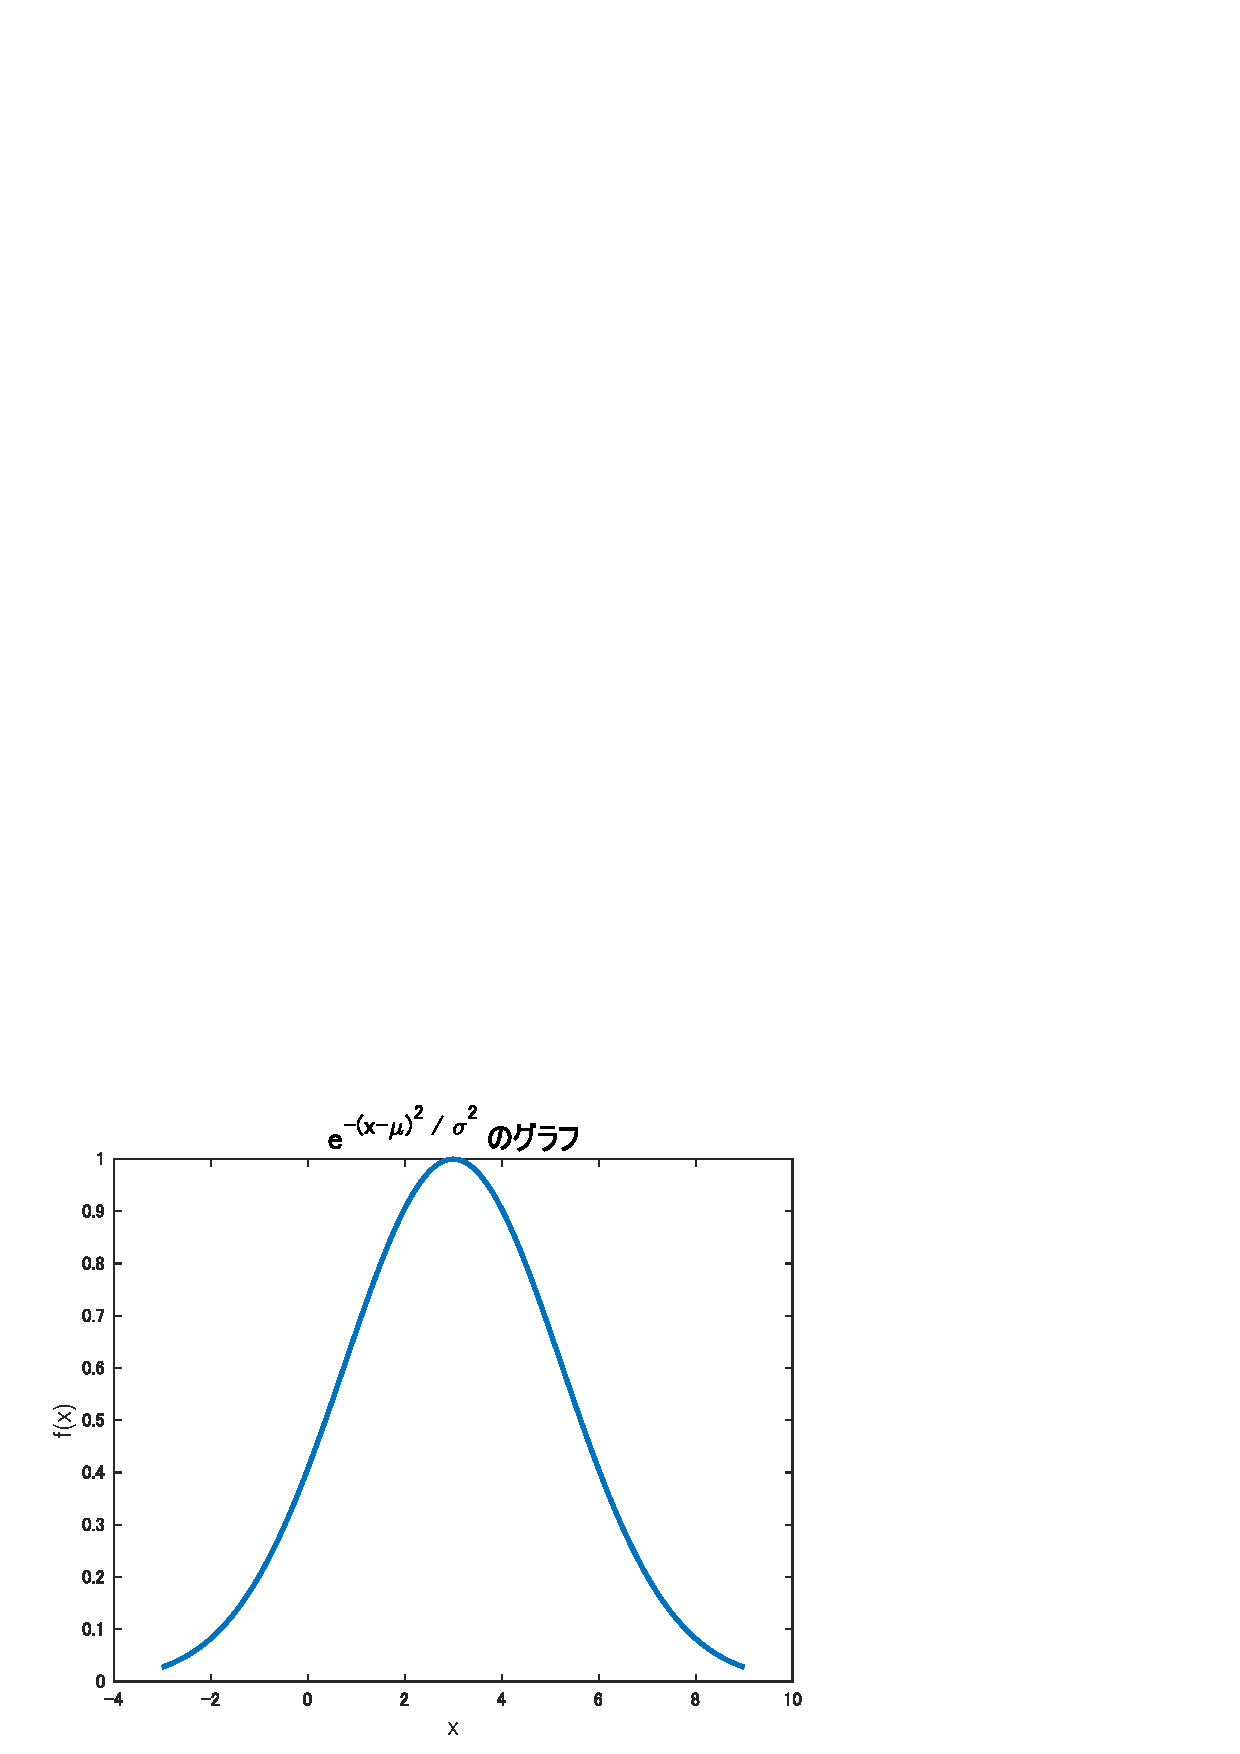
\includegraphics[width=120mm,bb=0 0 432 288]{../figures/normal4.png}
  \caption{式(\ref{eq:normal4})の図.(平均3, 分散10の場合)}
\end{figure}

え?式(\ref{eq:normal})と違うじゃないかって?\\
 せっかちだなぁ......余裕がない人間はモテないですよ.\\
\\
 まあ, グラフの形は実際これで完成なのです. ただ, 今我々が求めていたのは正規分布の「確率密度関数」でしたね?\\
\\
 確率の密度なのですから, 当然合計して1にならないといけないわけで, 先程の式(\ref{eq:normal4})ではその点がダメなのです. ちゃんと全確率点での値を足して1になるように正規化する必要があります.\\
\\
 つーわけで積分方程式を解きますがその前に, 出てくる計算結果を綺麗にするために式(\ref{eq:normal4})に細工をし, $\sigma^2$を$2\sigma^2$にしておきます. 2が付きましたが, グラフの性質自体は変わりませんね?\\
\\
 では積分方程式.
\begin{align}
\int_{-\infty}^{\infty} c e^{-\frac{(x-\mu)^2}{2\sigma^2}} dx= 1
\end{align}
を解きます...出来たものがこちらです.

\begin{align}
\label{eq:c}
c = \frac{1}{\sqrt{2\pi\sigma^2}}
\end{align}

式(\ref{eq:c})で得られたcを改めて式(\ref{eq:normal4}の変形版)に代入すると

\begin{align}
f(x) = \frac{1}{\sqrt{2\pi\sigma^2}}e^{-\frac{(x-\mu)^2}{2\sigma^2}}
\end{align}

が出てきましたね!良かった良かった. 以上が正規分布の確率密度関数の導出工程でした. フーリエなんかに比べれば雑魚ですね!ワンパンでした!\\
 え?積分方程式の解き方ですか?なんかMATLABにお願いしたら解いてくれました...

\subsection{100p\%点}
次. 正規分布を学ぶ意味は, この概念があるからといっても過言じゃない重要な性質です. 正規分布は平均が丁度真ん中で, 広がり方は分散によって定義される左右対称な特殊な分布でしたね?\\\\

つまり, 平均の周辺であるほど高確率で観測され, 裾野ほど「レア」な事象というわけです.\\\\

この性質を利用して, 正規分布には「100p\%点」と呼ばれる指標を導入する事が出来ます. これは「その点以上(以下)の部分の確率の合計がpになる境界」を指します. x軸の正方向なら上側, 負方向なら下側, 両方を指すなら両側100p\%点です. \\\\

言葉だとややこしいですが, グラフで見れば一瞬で分かります.


\begin{figure}[H]
\label{im:upper}
  \centering
  \includegraphics[width=120mm,bb=0 0 432 288]{../figures/upper_p.png}
  \caption{正規分布の上側5\%点}
\end{figure}

\begin{figure}[H]
\label{im:bilateral}
  \centering
  \includegraphics[width=120mm,bb=0 0 432 288]{../figures/bilateral_p.png}
  \caption{正規分布の両側5\%点}
\end{figure}

上側5\%に比べ, 両側5\%は左右に領域が分散した分上側の領域が狭くなってるのに注意です. \\
\\

だいたい, 正規分布でよく用いられるのは上下両側の5\%と1\%点です. 何に使うのかはあとで説明するので, ひとまず概念だけ覚えておいてください.

\section{t分布}
少ない標本数をもとに母分散がわかっていない母集団の母平均推定に使われるのがt分布です. 詳しくは推定の項で触れるので, ここでは確率密度関数と性質の確認をします.

\begin{align}
\label{eq:student}
f(x) = k(1 + \frac{x^2}{\alpha})^{-\frac{\alpha+1}{2}}
\end{align}

式(\ref{eq:student})がt分布の確率密度関数です. ここで$k$は定数, $\alpha$は自由度という指標で, この形を「自由度$\alpha$のt分布」と表現します. 自由度とは何かはここでは説明しませんが, 母集団によって算出できる値です. それ以外の部分では正規分布に似ていますね. 実際, 自由度$\alpha$が十分に大きい場合には正規分布になります. ただこいつの平均と分散は

\begin{align}
\mathbb{E}(X) = 0\\
\mathbb{V}(X) = \frac{\alpha}{\alpha-2}
\end{align}
です. 

\begin{figure}[H]
\label{im:student}
  \centering
  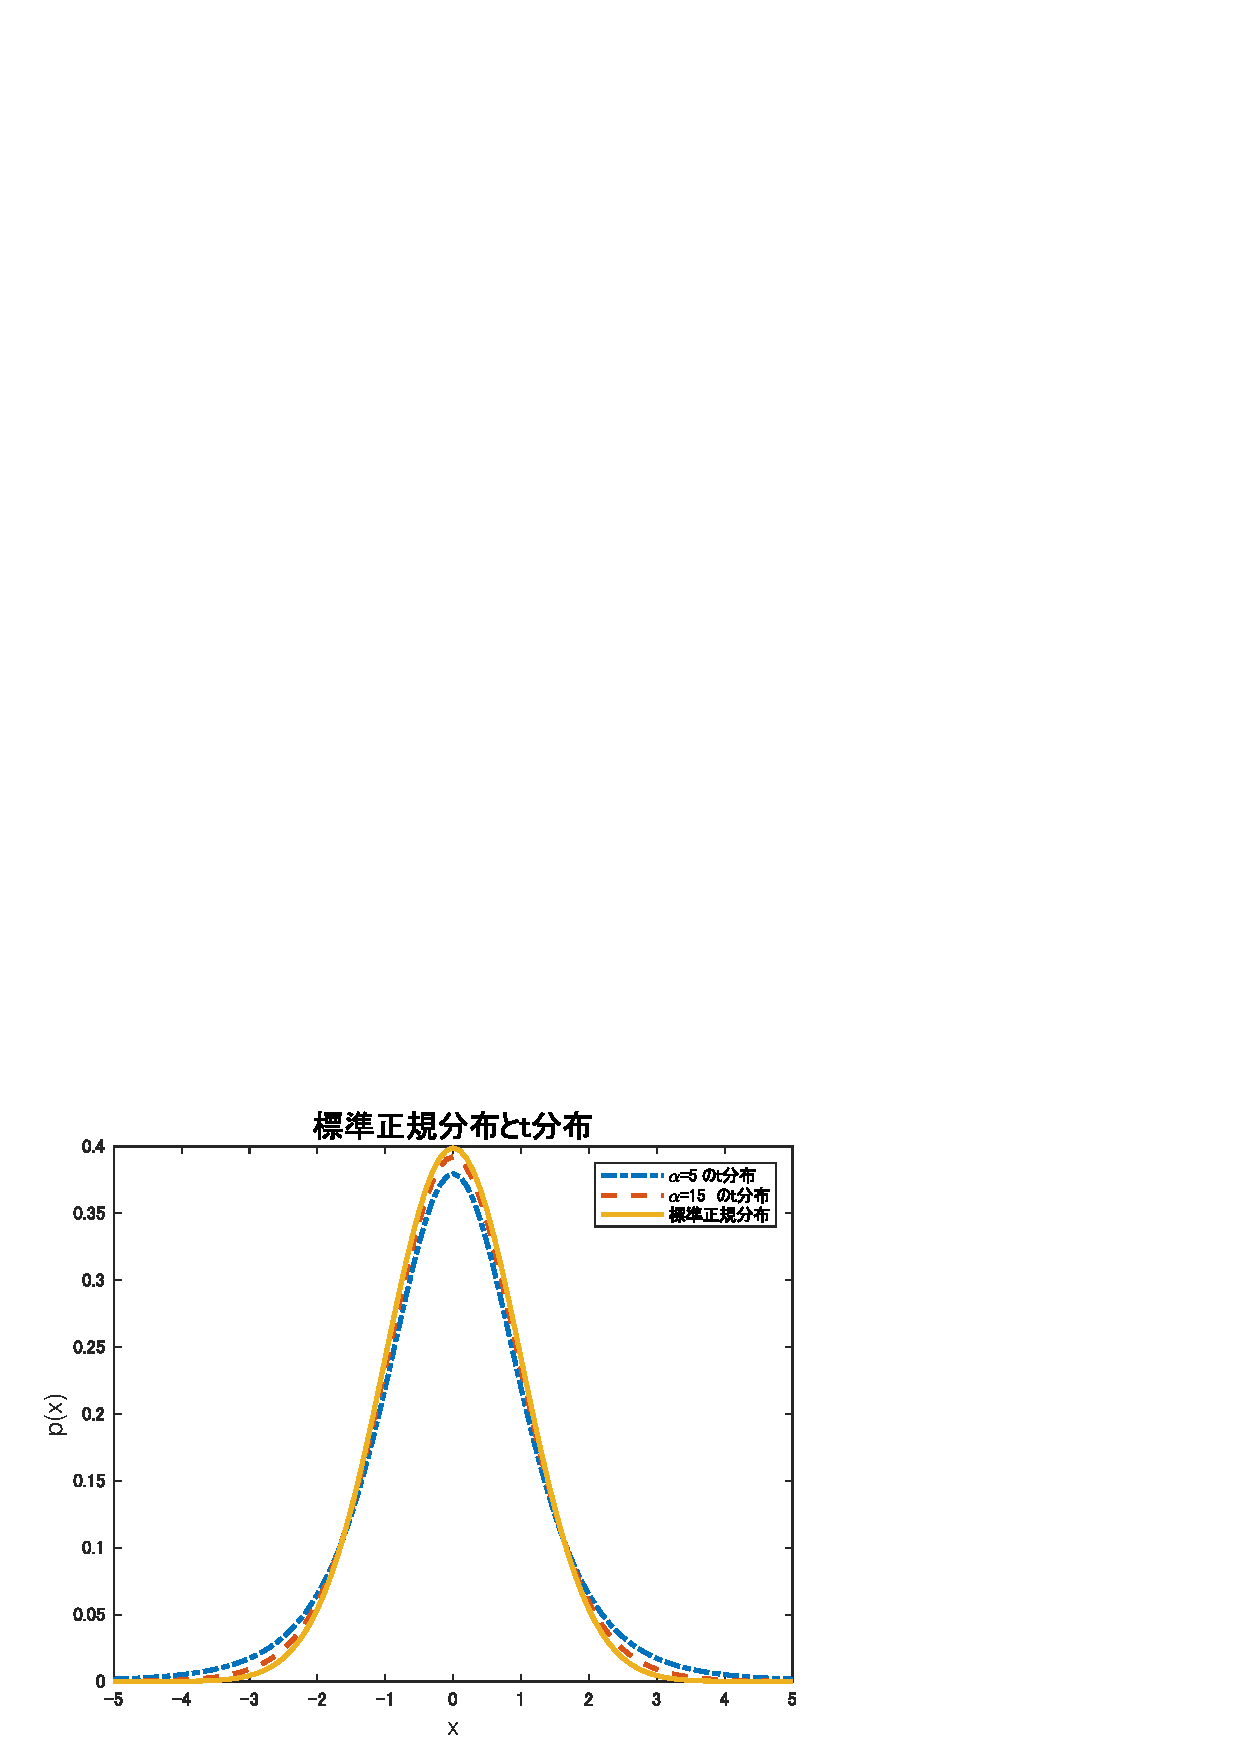
\includegraphics[width=120mm,bb=0 0 432 288]{../figures/student.png}
  \caption{自由度の異なるt分布と標準正規分布}
\end{figure}

自由度の異なるt分布と標準正規分布の比較です. 標準正規分布とは, 正規分布のうち平均が0, 分散が1のやつです. $\alpha$の値が大きいとほぼ同じ形になる事が分かると思います.\\
\\

では何に使うのかですが, そこはひとまず置いておきます. とにかくこういう分布があるのです.


\section{F分布}
F分布は, 少し特殊な形をしていますが非常に重要です. どう重要かというとF分布はこれまでの分布と異なり, 2つの母集団から得られた標本分散の比の確率分布になります. これの何がすごいのかというと, 例えば図(\ref{im:f_dist})は自由度が3の母集団Aと自由度が10の母集団BのF分布ですが, 「普通は」この組み合わせだと0から2あたりの値になる事が多いのです. \\
\\

しかしもし今, 自由度3と10のとある母集団A,B間でF値を取ったら6とかが出たとします. \\

通常はありえない値, つまり統計的に考えると「自由度だけでなく分散そのものに差がある = A,Bの母集団は異なる」となるわけですね. こちらも詳しくは後程. 式はえぐえぐです. 震えろ.

\begin{align}
f(x) = \frac{kx^{\frac{m}{2}-1}}{\{1 + (\frac{m}{n})x\}^{\frac{m+n}{2}}}
\end{align}

こいつの導出はいいです. 僕もわからん. 気が向いたら勉強してまとめるかも. 例によってkは定数, m,nは標本集団2つのそれぞれの自由度です. こいつは「自由度m,nのF分布」と表現されます. 今はそれだけ. 続いてグラフです. 幸いこっちは簡単.

\begin{figure}[H]
\label{im:f_dist}
  \centering
  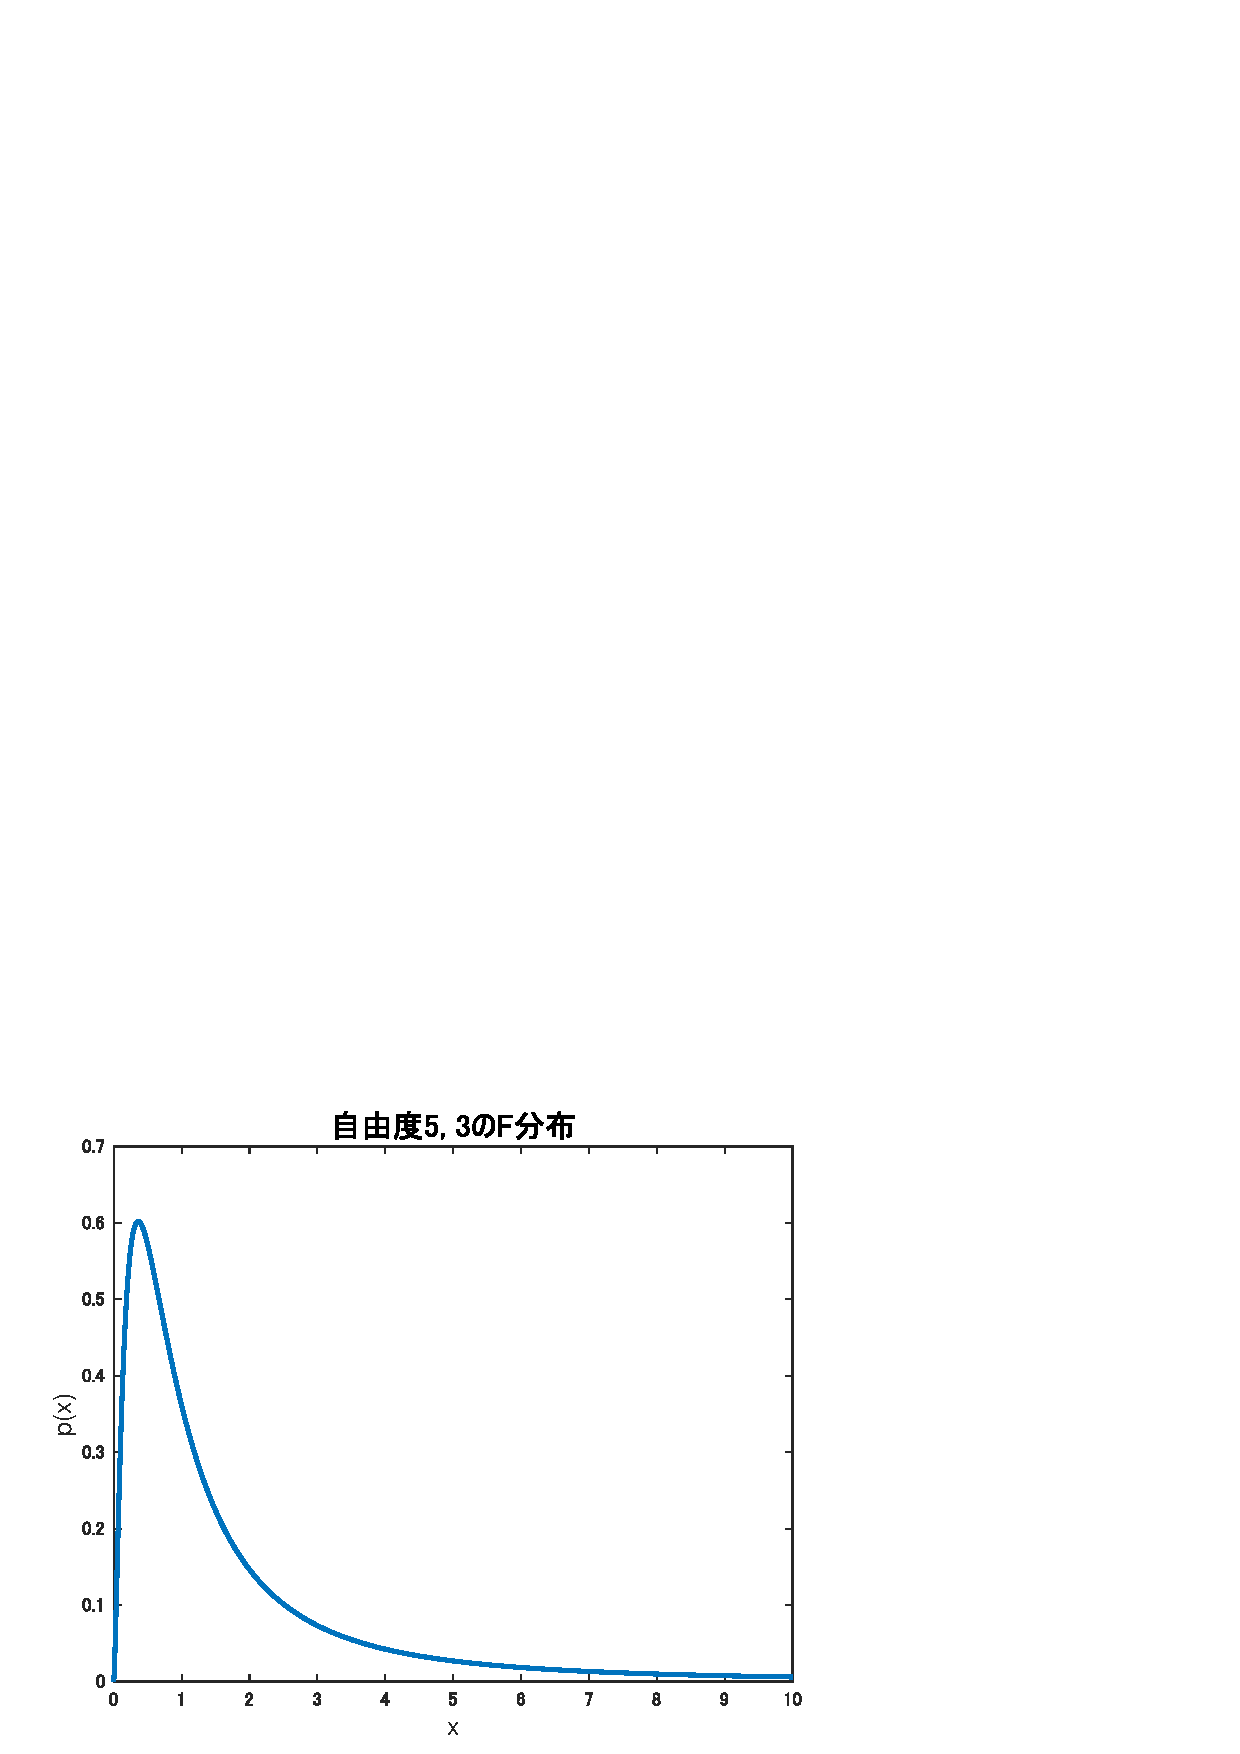
\includegraphics[width=120mm,bb=0 0 432 288]{../figures/f_dist.png}
  \caption{自由度3.10のF分布}
\end{figure}

恒例の平均値と分散です. こいつらも殺意高めだけど覚える必要は今のところ皆無だと思ってます.

\begin{align}
\mathbb{E}(X) = \frac{n}{n-2}\\
\mathbb{V}(X) = \frac{2n^2 (m+n-2)}{m(n-2)^2(n-4)}
\end{align}

\section{$\chi^2$分布}
ラスト. $\chi^2$分布です. こいつも重要です. 我々は結果を理論に落とし込む時, なんらかの数式に近似したり回帰したりするわけですが, 実際問題理論と観測値が完全に一致するなんていう事はまれで, 様々な要因で若干の誤差が生じます. その誤差が「誤差」なのか「理論の誤り」なのかを評価する時に使うのがこの分布とそれに基づく検定です. \\
\\
式はこちらです. 
\begin{align}
f(x) = k\chi^{\frac{\alpha}{2}-1}e^{-\frac{\chi}{2}}
\end{align}

またえぐえぐですね. えぐえぐと言えば, 筆者は声優の江口拓也さんが「やはり俺の青春ラブコメは間違っている」のラジオでやっていた「ぼっちラジオ」が大好きです. どうせこんな数学の同人誌読んでる人は陰キャだし, 楽しめると思います. 是非YouTubeで検索してみてください.\\
\\

さて, 例によってここの$\alpha$は自由度, kは定数です.\\

幸い, どこの説明を見てもこの式は使わないと言われているので覚えなくていいでしょう.\\
\\

平均値と分散です.
\begin{align}
\mathbb{E}(X) = \alpha \\
\mathbb{V}(X) = 2\alpha
\end{align}

簡単すぎワロタwwついでグラフです.


\begin{figure}[H]
\label{im:chi}
  \centering
  \includegraphics[width=120mm,bb=0 0 432 288]{../figures/kai.png}
  \caption{自由度の異なる$\chi^2$分布}
\end{figure}
 
こいつは結構F分布に似てますね. ただ注意が必要なのは, F分布は標本分散の比に関する分布ですが$\chi^2$分布は標本分散そのものの分布です.


\chapter{大数の法則と中心極限定理}
さて,こうして様々な確率分布の形を見てきたわけですが,そもそも全体のデータを観測して,そいつらの分布を見るならまだしも未知の集団の中から一部を抜き出して分布を見たところで,そいつの性質(平均とか)をどれだけ信じて良いものでしょうか.\\


\section{大数の法則}

よくある問題が,政党支持率を街頭インタビューやてきとうな電話で100人や1000人に聞いたデータを元に算出しているのはどれだけ信用できるのか問題とかですよね.「あんなたった100人に聞いただけじゃ信用できん!印象操作だ!」みたいな話になりかねません.そこで出てくるのが,大数の法則です.\\
\\

今,コインをn回投げて,その表が出る確率がちゃんと1/2なのかを確かめる作業を考えます.i回目の試行で表が出た場合1,裏の場合0を取る確率変数$x_i$を考えると,n回投げた時の表が出た回数は

\begin{align}
  r = \sum_i^n x_i
\end{align}

この量を頻度と呼び,更にこれを試行数nで割ったr/nを相対頻度と言います.rは確率変数なので,二項分布

\begin{align}
  f(x) = {}_n C_x (p)^n
\end{align}


に従います.こいつらの期待値と分散は二項分布のとこで確認したように

\begin{align}
  E(r) = np\\
  V(r) = np(1-p)
\end{align}

である事が分かります.相対頻度の期待値と分散は

\begin{align}
  E(r/n) = np/n = p\\
  V(r/n) = p(1-p)/n
\end{align}

となる事も分かると思います.で,こいつの試行数nの値を変えた時,E(r/n)の値がどう変化していくのかを見てみましょう.直観的,というか常識的に,n=3とかみたいに極端に試行数が少ないと信用できない事が分かるかと思います.逆に,n=1000000とかといった膨大なデータがあれば,そいつらがちゃんと分布の真の期待値であるpに収束する事が分かるでしょう.で,もしここでn=100とかで見ても全然収束してないのであれば,街頭インタビューで100人のデータを用いて結論付けられた発表は信じるに値しなさそうですね.\\
\\

では,コイン投げをしていきます.表が出る確率はちゃんと1/2としておきます.ここで,試行回数を変化させていった時それぞれに対応する,r/nの0.5付近(±0.1)の値を見ていきます.つまり,ちゃんと真の期待値に迫れているかという事を評価します.

\begin{align}
  P(0.4 \leq r/10 \leq 0.6) = 0.656\\
  P(0.4 \leq r/20 \leq 0.6) = 0.737\\
  P(0.4 \leq r/50 \leq 0.6) = 0.881\\
  P(0.4 \leq r/100 \leq 0.6) = 0.968
\end{align}

はい,という事で,nが増えるにつれて確率が上がっていき,真の確率(表が出る確率)に迫っている事が分かります.実際,もう100回もやれば十分ですね.というのが感覚的な説明でしたが,これを数式で表現すると以下のようになります.

\begin{align}
  P(|r/n -0.5| > 0.1) \longrightarrow 0\qquad(n\rightarrow\infty)
\end{align}

相対頻度が真の値である0.5から0.1以上離れている確率が0に収束していく過程,ですね.これこそが大数の法則(の一例)です.\\\\

では,より一般に大数の法則を導いて行きましょう.そのためには,チェビシェフの不等式というものが必要で,さらにそいつはマルコフの不等式をベースに考える必要があります.ということでまずはマルコフの不等式から行きましょう.

\subsection{マルコフの不等式}

\begin{screen}
  \textbf{マルコフの不等式}\\
  任意の確率変数$X$と$a>0$に対して
  \begin{align}
    P(|X| \geq a) \leq \frac{E[|X|]}{a}
  \end{align}
\end{screen}

これがマルコフの不等式です.よく分からんと思うのでまずは証明しましょう.確率変数Xに対して,ある範囲としてaがでてきてるのでXの期待値$E[|X|]$は以下のように書けます.

\begin{align}
  E[X] &= \int_0^\infty xf(x)dx \nonumber \\
  &= \int_0^a xf(x)dx + \int_a^\infty x f(x)dx
  \label{eq:mark}
\end{align}

式(\ref{eq:mark})のうち,第一項を意図的に消した場合,下のように変形されますね.Xは絶対値を取られるやつなので,第一項は必ず正の値を取っていることに注意です.

\begin{align}
  E[X] \geq \int_a^\infty x f(x)dx
\end{align}

ここで,xが取りうる範囲はaから$\infty$までとなっているので,この中で最小のaですべてのxを置き換えてみます.すると

\begin{align}
  E[X] &\geq a\int_a^\infty f(x)dx\\
  \therefore E[X] &\geq aP[X\geq a]
\end{align}

となります.何をやってるのかちょっと分からなくなってくるかもしれませんが,まずaから$\infty$でf(x)を積分してるんだからa以上の値をとる確率密度関数ですよね.で,こいつのa倍をしているものなので,$aP[X\geq a]$で書き換えられるわけです.したらこの式を移項して生理してあげればマルコフの定理,即ち

\begin{align}
  P[|X|\geq a] \leq \frac{E[|X|]}{a}
\end{align}

がでてきます.証明終わり.\\
\\

では肝心の,この不等式が何を指しているのかですが,まあ実際数字を入れてみれ考えれば分かると思います.さいころで考えてみます.出る値は1~6なので,期待値は3.5です.この時,aをたとえば1にした時,1より大きい値を取る可能性は当然高く,それは右辺が1で割られている事からも明らかです.が,3とかになると割った結果がほぼ1になりますね.3.5/3だから.雲行きが怪しくなってきました.さて,ここに5なんかを入れると,もはや分母の方が大きいので,値は1よりも小さくなります.一方の左辺も,aの値が大きくなるにつれて取れる値の範囲が狭くなっていくので,それらの値を取る確率もやはり下がっていきます.\\
\\

この関係を表すのがマルコフの不等式でした.

\subsection{チェビシェフの不等式}
ふう.マルコフの不等式が分かれば,チェビシェフの不等式なんてワンパンです,ワンパン.秒で沈めてやりましょう!

\begin{screen}
  \textbf{チェビシェフの不等式}\\
  期待値$E[Y] = \mu$, 分散$V[Y] = \sigma^2$とするとき,任意の実数 $k>0$ に対して
  \begin{align}
    P[|Y-\mu| \geq k\sigma] \leq \frac{1}{k^2}
    \label{eq:cheb}
  \end{align}
  が成り立つ
\end{screen}

めちゃくちゃ見覚えありますね.そう,これはマルコフの不等式の特別な場合を考えればすぐ証明できます.\\

まずマルコフの不等式において,$X=(Y-\mu)^2, a = k^2\sigma^2$とすると

\begin{align}
  P[(Y-\mu)^2 \geq k^2\sigma^2] &\leq \frac{E[(Y-\mu)^2]}{k^2\sigma^2}\\
  \therefore P[|Y-\mu| \geq k\sigma] &\leq \frac{1}{k^2}
\end{align}

となります.ただしここで,$E[(Y-\mu)^2]=\sigma^2$を使っています.\\\\

さて,こいつの何がすごいのかを考えてみます.結論からすると,チェビシェフの不等式がそのまま大数の法則を示すものになっています.というのも,まず式(\ref{eq:cheb})を見てみると「得られたデータが,$k\sigma$以上離れた位置,正規分布とかで考えるならめっちゃ裾の方ですね,を取る確率」である左辺は,$k^2$の逆数以下になるよって話ですね.\\
\\

たとえば,あとで出てきますが正規分布の時によく使う$3\sigma$以上の値を取る確率は0.3\%程度なのですが,実際この値($1/k^2$)は1/9なので0.3以下になりますね.\\
\\

すごいのは,得られたデータがどんな分布に従っていたのかという母集団の情報が全くなくても,こいつの収まる範囲が分かる事です.どんな分布でも絶対,$1/k^2$以下になるってわけですね.正規分布の時実際そうなるのは上で確認した通り.めっちゃすごいっすねこれ.分布知らなくても言えるわけですからね!!

\subsection{大数の法則}
で,肝心の大数の法則です.証明していきます.
チェビシェフの不等式の証明において,k=$a^2$としてみると,
\begin{align}
  P[|X-\mu| \geq a] \leq \frac{\sigma^2}{a^2}
  \label{eq:cheb2}
\end{align}

となります.これも計算自体は全く同じなので,チェビシェフの不等式と呼ばれます.ここで標本平均$\bar{X}$を考えると,$E[\bar{X}] = \mu, V[\bar{X}] = \frac{\sigma^2}{n}$となります.これを式(\ref{eq:cheb2})に代入すると

\begin{align}
  P[|\bar{X}-\mu|\geq a] \leq \frac{\sigma^2}{a^2n} \xrightarrow{n\rightarrow\infty}0
\end{align}

となると思います.良いでしょうか.nの値が大きくなるにつれ,右辺の分母が大きくなるので値は0に収束していくわけですね.そう,これが大数の法則です!!\\
\\

nの値,つまり得られた標本の数($\bar{X}は\sum X_i/n$)が多くなるほど,真の値との誤差は0に向かって小さくなっていくことを指しています.\\\\

その主張することは何かというと,こうです.\\

\textbf{「大標本では,観測された標本平均を母集団の真の平均とみなしてよい」}\\
\\

これがあるからこそ,我々はある程度のサイズのデータを使って一般化した議論が出来るわけですね.しっかり確認しておきましょう.


\section{中心極限定理}
大数の法則同様,統計学においてとても重要な定理としてもう一つ,中心極限定理があります.というかこちらの方がどちらかと言えば大事かも.定理は以下です.\\

\begin{screen}
  \textbf{中心極限定理}\\
  期待値$\mu$,標準偏差$\sigma$の分布に従う確率変数列$X_1,X_2...X_n$に対し,$S_n := \sum_{k=1}^n X_k$とすると
  \begin{align}
    P(a \leq \frac{S_n -n\mu}{\sqrt{n}\sigma} \leq b) \xrightarrow{n\rightarrow\infty} \int_a^b \frac{1}{\sqrt{2\pi}}e^{-\frac{x^2}{2}}dx
  \end{align}
  が成り立つ.
\end{screen}

はい,なんも分からんと思います.\\
\\

ここで言いたいのは,与えられたデータから求めたそれぞれの標本平均$X$の総和である$S_n$を標準化(左辺の真ん中のごちゃごちゃしたやつ.平均を引いて標準偏差で割ってる)したやつはnが十分に大きいと,つまり得られるデータが多いと,期待値0,分散1の正規分布に収束するということです.\\

正規分布の確率密度関数は以下でしたね.

\begin{align}
  f(x) = \frac{1}{\sqrt{2\pi\sigma^2}}e^{-\frac{(x-\mu)^2}{2\sigma^2}}
\end{align}

ここで$\mu$を0,$\sigma$は1を代入した形が中心極限定理の右辺に来ています.こいつをaからbの範囲で積分したものが,標準化変数である左辺の項がaからbに収まる確率と同等になるという事を表していますね.

即ち,nが十分に大きいなら部分和である$S_n$は平均が$n\mu$,分散が$n\sigma^2$の正規分布に従う事になり,よって標本平均である$\bar{X_n}=(X_1+...+X_n)/n$も平均$\mu$,標準偏差$\sigma/\sqrt{n}$に従う事になります.\\
\\

大事なのは,今回定理のところでそもそも,母集団の分布を何も仮定していないところです.大数の法則同様,母集団の分布に関わらず従う法則なわけですね.\\

\textbf{母集団がどんな形であれ,nが大きい時にはそこから得られた標本平均は正規分布に従う}という性質を意味します.\\
\\

ゆえに,正規分布は数ある確率分布の中でも最も重要な分布と言われるわけですね.今後学んでいく様々な検定や推定なども,正規分布を仮定する事が多いのはこれが理由になっています.\\
\\
\\

(証明...モーメント関数とか必要で自分がちゃんと整理しきれてないのと,どこにその説明いれるべきなんや...てか必要かな...と悩んでしまっているのでとりあえず保留!ごめんなさい!!)

\chapter{統計的検定}
今の今まで,面倒だなあ面白くないんだよなあと逃げに逃げまくっていましたが...「はやく検定書けよ使えねえオタクだな」って色々な人に尻を蹴りあげられたので,その勢いで腰をあげて頑張ろうと思います.\\

しかしまぁ,最近の神経科学というか実験心理学では統計の問題が色々と指摘されていて,日々Twitterで神経科学のキラー細胞みたいな御仁が色々な人の研究を晒上げて燃やし尽くしている状況なので,統計の記述をするのマジで怖いですね...自浄作用を働かせるのは大事だけど,それはあくまで界隈の発展のためであって他者を攻撃して気持ちよくなるためのものではないと思うのでもう少し考えてみてほしいものですね.


さて,がんばるぞい\\

\section{統計的仮説検定とは}
統計的仮説検定とは何か,いつ使うものなのかですが,結論から言えばどの論文にもほぼ必ず出てくる作業ですよね.研究者の掲げる「ある仮説」の有意性を検定するものです.「ある仮説」の元で期待する結果と,実際に得られて観測された結果とを見比べた時,そこにある差が偶然起こった程度のものだと言えるか,否かを評価します.偶然じゃないのなら,きっとその差には何か意味があるはず,つまり仮説が間違っているという事になります.\\

これを使って,たとえば1軍と2軍の能力は同等であるという仮説の元に能力テストを行って,結果を比べると明らかに1軍の方が高かったとなれば,残念ながら仮説は間違っていて1軍より2軍の方が優秀であったんだ!のような主張を出来るわけですね.\\

この発想自体は,我々人間が日頃からやっているようなごく普通の思考プロセスですよね.\\

与えられた仮説のもとで考えられる範囲を超えた誤差が生じた場合,それは何らかの意味があると考え,このずれは「有意である」,と言います.ここから,統計的仮説検定とは即ち仮説の有意性検定であるとも言えます.\\

ではここで問題なのが,どうやってその有意性を判断するのかです.有意性とは,標本が有意なずれを示す確率であるので,ここで標本分布を使う事になります.コインを10回投げて,表が何回出るかを使ってコインがいかさまコインじゃないかを判定する事を考えましょう.一般のコインであれば,確率的に平均を取れば5回表が出るはずですね.

5回表が出たら,普通の人ならイカサマコインではない判定をすると思います.では4回ならどうでしょう?たった10回の試行中なので,僕なら良しとします.では3回は?ここらへんから少し怪しいですね...僕は何とも言えないなぁくらいの評価です.2回まで行くと,ちょっとイカサマを疑っちゃいますね.1回とか0回は舐めてる.許せんわ.\\\\

と,普通に我々が行う思考はこんな感じですね.表が出る確率pは$p(表)=1/2$であると考えて,二項分布($Bi(10,1/2)$)の確率分布に従う事を仮説として,その中で与えられたデータ(表が出た回数)が分布のどのあたりにあるのかを考えるわけです.

\begin{figure}[H]
  \label{im:bino}
    \centering
    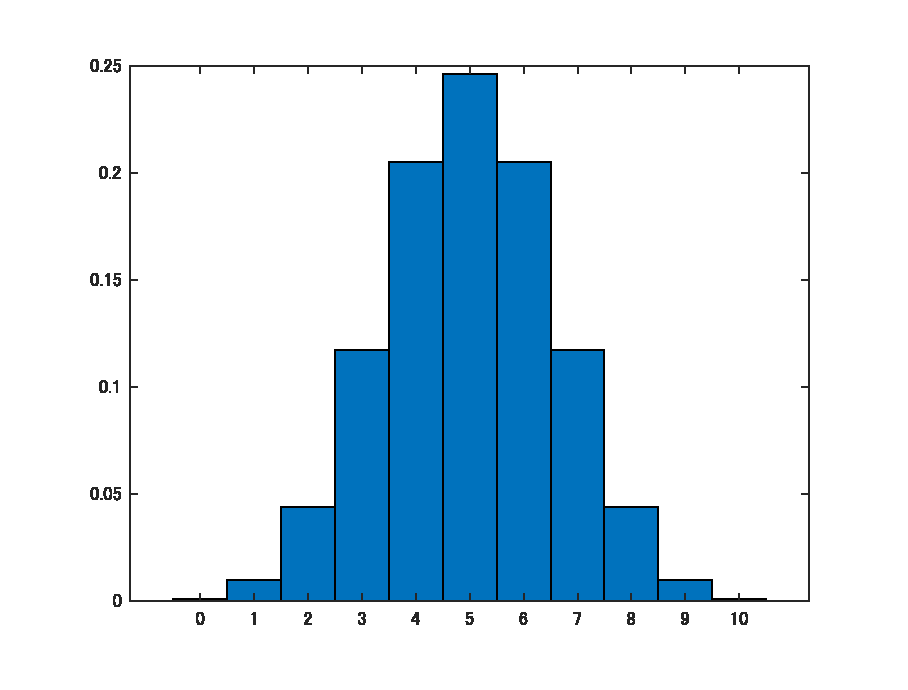
\includegraphics[width=120mm]{../figures/bino.eps}
    \caption{表が出る回数の二項分布}
\end{figure}

確率の議論なので,ここでさっきの例をちゃんと計算してみましょう.n=10の2項分布で表が出る回数別にそれぞれの確率を計算すると以下のようになりました.

\begin{align}
  x=5 \qquad p = 0.2461 \nonumber \\
  x=4 \qquad p = 0.2051 \nonumber \\
  x=3 \qquad p = 0.1172 \nonumber\\
  x=2 \qquad p = 0.0439 \nonumber
\end{align}

こう見ると,やはり3あたりから怪しくて,2はやばいってのがなんとなく分かりますね.2回だけ表が出る確率は二項分布の元でわずか4.3\%しかないわけですからね.\\
\\

この時,仮説の元では出るはずがない結果がでたということで,仮説が誤っていたと判断します.この事を,仮説を棄却する,と言います.\\

また,実用では基本的にこの仮説は否定したい,というか否定される事を想定して設定されるものです(研究であれば,AグループとBグループに差があると言いたいから,差がないという仮説を立てて否定しますね).故に,こうして否定される仮説の事を特に,帰無仮説とも言います.\\

反対に,対立的な仮説(コインの例なら,表が出る確率は1/2未満である,とか)を立てて置くこともあります.この仮説を特に,対立仮説と言います.\\

帰無仮説と対立仮説は互いに反する事象なので,帰無仮説を否定する事は対立仮説を採択する事とほぼ同義,というふうにして使われる事が多いですね.がしかし,注意が必要なのは帰無仮説が$p=0.5$だとして,対立仮説に$p<0.5$を置いたとしたら第三の可能性として$p>0.5$もあります.こうした場合は帰無仮説の否定=対立仮説の採択とは違うので気を付ける必要があります.\\


以上の内容を言い換え,改めて仮説検定とは何か考えると,\\
「用意された仮説が有意であるか否かを判断し,それに応じて仮説を棄却するか採用するか判定する作業」\\
であると言えます.\\
\\
\\

ここまでの内容で,ある程度くらいの脳を持った人なら気付くと思いますが,確率やらを持ってきてそれっぽい空気を出してはいるけど結局最後の有意性の判定が恣意的でしたよね.さっきは「わずか4.3\%しか起こりえないはずの事象を観測するのはおかしい」と決めつけて,コインはイカサマであると判断しました.\\

その時々の気分で勝手に変えるのも困るので,こうした有意性の判定のためにある基準値を設ける必要があります.それが有意水準($\alpha$)と呼ばれるやつです.\\

ほら,よく論文とかでも見る$p<0.05$とかのやつです.これはp値が0.05という有意水準を下回っていますよ,つまり有意ですよ,だから帰無仮説を棄却しますよ,という意思表示なわけですね.一般に,有意水準は0.1,0.05,0.01などが使われます.\\
\\

しかし有意水準を下回ったからといって,絶対にありえないわけじゃありません.5\%の確率でしかありえない事は,20回に1回程度は起こりうる事でもあります.そのため,帰無仮説や対立仮説をそれぞれ採択したけれども,実際は誤りで他方が正解であったという事が起こってしまいます.
これらの誤りをまとめると以下のようになります.

\begin{figure}[H]
  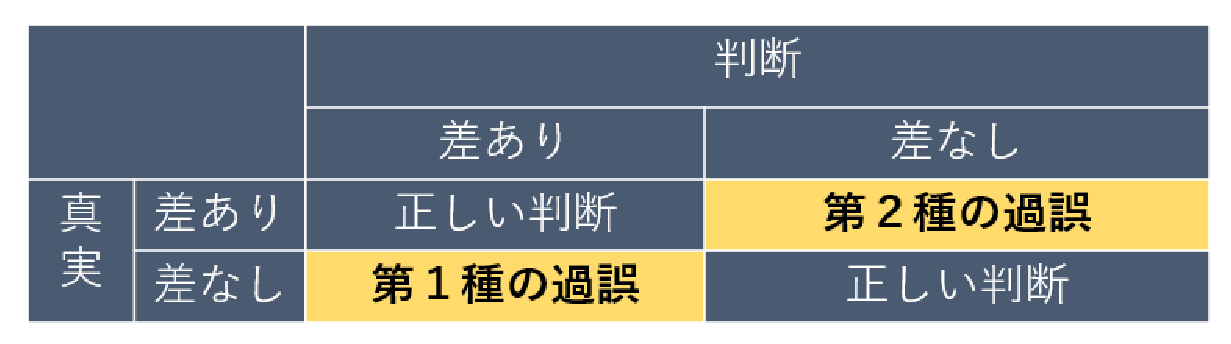
\includegraphics[width=15cm]{../figures/miss.eps}
  \caption{統計的仮説検定の結果と過誤の対応}
\end{figure}

帰無仮説を棄却したけど実際は偶然で5\%とかの確率を引き当ててしまっていた場合を第一種の過誤,帰無仮説を採択したけど実際は仮説が間違っている場合を第二種の過誤と言います.\\

また,第一種の加護は偽陽性,第二種は偽陰性とも言います.個人的にはこっちのが分かりやすくて好きです.

もう一つ注意が必要なのは,統計的仮説検定は帰無仮説が否定される事によって対立仮説を採択するといういわゆる背理法を用いているので,厳密には帰無仮説が棄却されなかったからと言ってそれが正しいという事にもならないし,対立仮説が間違っているとも言えません.あくまで,帰無仮説と得られた結果が矛盾しない,というだけにとどまります. \\\\

以上の性質を踏まえ,検定の用いる目的として主に3つの状況が考えられます.\\

\begin{itemize}
  \item 帰無仮説を反証し,棄却する目的
  \item 異常の検知
  \item 数学的に扱いやすいためおく便宜的な仮定
\end{itemize}

まず一つ目,これが最も我々が使うものかもですね.先に説明したように背理法的な使い方をして,データに見られる誤差が確率的に偶然で許される範囲かを考え,逸脱していた場合は帰無仮説を棄却して対立仮説を採択するやつ.新薬の効果があるって主張したいから,まずは薬を投与してもしなくても変わりませんよって帰無仮説を設定してそいつを論破してやろうって使い方です.\\

次に二つ目,異常の検知です.こいつも検定の例だとよく出てきます.本書でも書くと思うけど,工場の生産品の不良品率の話が例によくでてきますね.通常の状態であれば観測されるデータが属しているはずのデータ群として帰無仮説を設定しておいて,こいつが棄却されないならヨシ,されてしまうのなら何か異常があるとするやつです.\\

最後がちょっと特殊ですが,統計モデルを考える際に使うものぽい.確率変数が正規分布に従うって仮定をいろんなところで置くと思うんですけど,まあこれは中心極限定理があるからある程度信用できるとは家やはり分からない事なので,あくまで仮定は仮定,仮説です.なので,仮説検定を使ってちゃんとデータがこの分布に従っているのか,つまりここで置いたモデルは妥当なものなのかを検証する際にも使うことが出来ます.便利ですね.

\section{詳しく説明}
と,ここまでの内容は皆さん大体,既に知ってると思います.個人的な話になりますが,統計を勉強する上で特に検定でやる気が起きないの,とにかく数式での説明がないからよく分からないというかイメージしきれないってところなんですよね.という事で,以上の内容を数式使って表していきます.

まず,検定の問題では帰無仮説と対立仮説を置いていました.こいつらは相反するべきものなので,以下のように定義します.

\begin{align}
  \Theta = \Theta_0 \cup \Theta_1, \Theta_0 \cap \Theta_1 = \emptyset \text{(空集合)}
  \label{eq:hypo}\\
  H_0: \theta \in \Theta_0 vs. H_1:\theta \in \Theta_1
  \label{eq:vs}
\end{align}

ここで,式(\ref{eq:hypo})では$\Theta$は母数空間であり排反な部分集合である$\Theta_0, \Theta_1$に分けられています.こいつらがそれぞれ帰無仮説と対立仮説に対応する母数の集合です.ここで,未知のパラメータである$\theta$がそのどちらに属しているかを表すのが式(\ref{eq:vs})あり,これが帰無仮説と対立仮説(H)に相当します.\\\\

例で考えます.ある工場の製品の不良生産品率をpとしたとき,それが許容範囲かどうかを検定する問題で, pがある$p_0$以下であればヨシ,それを超えている場合には生産工程に問題があるとして責任者を減給する事にしましょう.さらに,一般に帰無仮説は$\Theta_0$,対立仮説は$\Theta_1$とする事が多いようなので従うと,ここで考える検定問題は

\begin{align}
 H_0 :p\leq p_0 \quad vs. \quad H_1 :p> p_0 
\end{align}

となりますね.閾値として設定した$p_0$を以下だったら有意さなし,セーフ,許すとして,超えていたら対立仮説を採択,この工場は問題ありとするわけです.\\
\\

それから前節で説明を忘れていた大事な概念に,両側検定と片側検定があります.これは検定問題の式を考えると分かりやすいですが,

\begin{align}
  H_0:\theta = \theta_0\quad vs. \quad H_1:\theta \neq \theta_0
\end{align}

のように,特定の値を決めてそれぴったしなのが帰無仮説,そうでない場合を対立仮説とする場合を両側検定と言います.つまり,分布の右でも左でも関係なく,とにかく帰無仮説で定めた値から逸脱した範囲の場合対立仮説を採択するものです.\\

一方で,

\begin{align}
  H_0:\theta \leq \theta_0 \quad vs. \quad H_1 : \theta > \theta_0
\end{align}

のように(あるいは不等号が逆でも),決めた値に対してどちらかに超えた場合を検出するものを片側検定と言います.たとえば,ある薬の治療効果を確かめたいという目的で検定をするなら,なんらかの健康の指標が薬の投与によって上昇すれば良いので,上側の片側検定で良さそうですね.このように目的に応じて検定は使い分けられます.\\\\

で,我々?検定を使う人?がやる決定dは,$H_0$が正しいのか$H_1$が正しいのかを判断する事です.帰無仮説$H_0$を採択する事をd=0,棄却する事をd=1としておきましょう.\\

すると決定の結果生じる損失について次のようにまとめられます.これを使って偽陽性や偽陰性について考えていきます.\\


\begin{align}
  L(\theta, d=0) &= \left\{
    \begin{array}{l}
    0, \quad if \quad \theta \in \Theta_0\\
    1, \quad if \quad \theta \in \Theta_1
    \end{array}
  \right.\nonumber \\
  L(\theta, d=1) &= 1-L(\theta, d=0) 
  \label{eq:cost}
\end{align}

損失関数については統計編で触れてないと思いますが,まあ「状況」と「判断」を変数としたときの,間違いによって生じる「損失」についての関数です.判断があってれば損失は生まれないし,間違っていれば生まれます.

ここでは,偽陽性や偽陰性の時に損失が生じれば良いわけですね.たしかに式(\ref{eq:cost})では正解が$\Theta_0$なのにd=1,つまり$\theta \in \Theta_0$を否定しちゃったり,逆に$\Theta_1$なのにd=0として$\theta \in \Theta_1$を否定しちゃったりしたときに1を取る,つまり損失が生まれる事になっていますね.\\

そう,偽陰性や偽陰性とはつまり,こうして判断の結果損失が生まれてしまう状態を指します.より一般には,偽陽性と偽陰性はどちらも同じ損失である必要はなく,偽陽性よりも偽陰性の方を厳しくみたいとか色々あると思いますが,ここではとりあえず等価としています.


\section{t検定}









\newpage
\chapter{ベイズ統計}
\section{頻度主義とベイズ主義}
これに触れるのは気が引けるというか,ややこしいのですがどの統計本もこの話題から触っているので一応.確率を考える方法には,どうやら ``主義''があるようです.確率や統計はその性質上,絶対的な正解というものは存在しません.「こんな傾向があるよね」なんて議論を数学的にやろうという話なので,絶対はないからです.それ故,考え方の基礎というか根っこの部分で置く仮定のようなもので派閥が別れるのかななんて思っています.\\

とかく,確率には頻度主義と呼ばれる派閥とベイズ主義と呼ばれる派閥があります.この派閥という表現だと対立しているようにも思えますし,実際対立している面倒な人達もいるようですが実際の現場ではどちらも便利なところがあるし,要は使い分けだと思います.よってどちらが優れているとか,どちらが正解とかいう議論は無意味だし,答えもないと思います.注意してください.\\
\\

ということで,筆者はこうした宗教戦争には興味がないのと下手に触れると炎上しそうなので紹介だけです.興味があるようなら自分で勉強してみてください.正直自分はよく分かってないです.

\section{加法定理と乗法定理}
ベイズ統計に入る前に,確率に関する基本的な法則を二つ導入しておきます.加法定理と乗法定理です.三角関数とかでおなじみのあれです.確率の加法と乗法について考えてみましょう.\\
\\

まずは加法定理から.確率変数$X,Y$を導入します.それぞれ$X=x_i, Y=y_j$を取る確率を$p(X=x_i, Y=y_j)$と書き,これを$X=x_i, Y=y_j$の同時確率と言います.\\

ここまでは良いですよね.$x_iとy_j$が同時に観測される確率だから同時確率です.\\
\\

さて,この$X, Y$の両方についてそれぞれサンプルを取る作業をN回行う事にします.この時,$X=x_i, Y=y_j$となる試行の回数を$n_{ij}$と表します.こうすると,以下の式が成り立ちますね.

\begin{align}
\label{eq:prob1}
p(X=x_i, Y=y_j) = \frac{n_{ij}}{N}
\end{align}

これは普通に,「大小のさいころ2つを振って大3,小6を引く確率(同時確率)を求めよ」とかと同じです.全試行分の当該試行ですね.
\\

では次に,$X=x_i$となる確率を考えます.Yが取る値と関係なく,$X=x_i$となる試行数を$c_i$としておきましょう.そうすると,$p(X=x_i)$は

\begin{align}
\label{eq:prob2}
p(X=x_i) = \frac{c_i}{N}
\end{align}

になります.「大小2つのさいころを振って,大きい方が6になる確率は?」です.うーん?この例あまり良くないですね.どちらにせよ試行数1なので...まあいいや.\\

この式(\ref{eq:prob2})ですが,式(\ref{eq:prob1})を使ってあえて複雑に書けばこうなります.

\begin{align}
\label{eq:sum-rule}
p(X=x_i) = \sum_{j=1} p(X=x_i, Y=y_j) = \sum_{j=1} \frac{n_{ij}}{N}
\end{align}

Yの値はなんでも良いから,Xが$x_i$になる確率を出したのが式(\ref{eq:prob2})なので,これは全ての$Y=y_j$について式(\ref{eq:prob1})を足し合わせたものと同じだよねという式になります.\\
\\
 これが確率の加法定理です.また,捉え方を変えるとこの処理はx以外の変数(ここではy)についての周辺化をするとも言い,式(\ref{eq:sum-rule})をxの周辺確率とも言います.\\
\\
 次に,$X=x_i$が既に観測されている状況に限って,その中で$Y=y_j$が観測される可能性を考えます.これを条件付き確率と言い,今の例だと以下のようになります.

\begin{align}
\label{eq:conditional}
p(Y=y_j | X=x_i) = \frac{n_{ij}}{c_i}
\end{align}

左辺の記法,最初は慣れないかもしれませんが慣れましょう.縦線は条件付きである事を表し,「右側の条件の元の左についての~~」を意味します.逆にならないように注意.筆者は最初よく逆に捉えていてわけわからんになっていましたが,これ以降頻繁に出てくる表現です.ここでは,上で述べたように ``$X=x_iの時のY=Y_iの確率(p)$''という意味です.\\
 式に戻りますが,右辺は分母に$X=x_i$になる試行数である$c_i$が来ていて,分子はXとYが$x_i, y_j$になる試行数である$n_{ij}$ですね.言葉の通り,$X=x_i$が確定した状況での$Y=y_j$が成り立つ可能性になっている事が分かるかと思います.\\
\\
 以上の事から確認されるように,加法定理同様,式(\ref{eq:prob1},\ref{eq:prob2})を考慮すると

\begin{align}
p(X=x_i , Y=y_j) = p(Y=y_j | X=x_i)p(X=x_i)
\label{eq:product}
\end{align}

が言えます.つまり,$X=x_i , Y=y_j$の同時確率は$X=x_i$が観測された上での$Y=y_j$の確率であり,これらの乗算によって求められるという事です.一応計算しても,

\begin{align}
p(Y=y_j | X=x_i)p(X=x_i) = \frac{n_{ij}}{c_i}\frac{c_i}{N} = \frac{n_{ij}}{N}
\label{eq:product}
\end{align}

で式(\ref{eq:prob1})が確かに求められていますね.これが確率の乗法定理です.意味するところは,$X=x_i, Y=y_j$の同時確率は$X=x_i$の確率と,$X=x_i$の元での$Y=y_j$の条件付確率との積である,ということになります.
\\
 まとめると,確率論の基本法則2つは以下になります.

\begin{screen}
確率の基本法則
\begin{align}
p(X) = \sum_Y p(X,Y) \qquad \text{加法定理} \nonumber \\
p(X,Y) = p(Y|X)p(X) \qquad \text{乗法定理} \nonumber
\end{align}
\end{screen}

ここでp(X)は確率変数Xの確率分布を指します.なので先程までの記法に従うと$p(X=x_1, x_2, x_3, ..., $となります.面倒なので以降はこうやって省略します.

\section{ベイズの定理}
いよいよベイズに行きます.ここではベイズ統計の歴史だとか主義がどうとかは一切触れないので,ぬるっと導入していきます.筆者がベイズいまいち分からん気がする理由は,ここでぬるっと導入できちゃうところにあったりもします.つまり主義がだの仮定がだの言っている割に,いわゆる頻度統計(?)で使ってる普通の式の変形でだせちゃうんですよね.いきます.\\
\\
 まず,同時確率は対称です.つまり$p(X,Y) = p(Y,X)$です.式(\ref{eq:prob1})より自明ですね.この性質を使って遊んでいるとベイズの定理が出てきちゃいます.

\begin{align}
\label{eq:bayes}
p(X, Y) &= p(Y|X)p(X) \\
\therefore p(Y|X) &= \frac{p(X,Y)}{p(X)}  \\
\therefore p(Y|X) &= \frac{p(X|Y)p(Y)}{p(X)} \qquad \because p(X,Y) = p(Y, X)
\end{align}

できちゃいました.$\therefore, \because$の使い方あってるかな?あってるよね.$\therefore$はtexだとthereforeって書き,$\because$はbecauseって書きます.これで分かりますね?\\
\\
 さて,あっさりとベイズの定理が出せちゃったわけですが,その意味を解釈する前にもう一つ導きたい式があります.分母にいる$p(X)$に関して,加法定理と同時確率の対称性を使って

\begin{align}
\label{eq:bayes-x}
p(X) = \sum_Y p(X,Y) = \sum_Y p(Y,X) = \sum_Y p(X|Y)p(Y)
\end{align}
が言えますね.これを使って書き直した特殊な表現と原型を以下にまとめます.

\begin{screen}
ベイズの定理
\begin{align}
p(Y|X) &= \frac{p(X|Y)p(Y)}{p(X)}\\
p(Y|X) &= \frac{p(X|Y)p(Y)}{\sum_Y p(X|Y)p(Y)}
\end{align}
\end{screen}

上の式がよく見るベイズの形.下は式(\ref{eq:bayes-x})を使って定義しなおした式です.下を使って,ベイズの定理の意味するところを見ていきましょう.右辺の分母は,分子の計算を全てのYについて足し合わせたものになっています.つまりこれは,左辺の条件付確率を全てのYについて足し合わせると1になるように正規化しているのだという事がわかります.確率だもんね,Aである確率は60\%,Bである確率が90\%,あわせて150\%です!なんてあほな話は困ります.\\
 大小2つのさいころの例で考えるなら,こんな感じ


\begin{align}
p(小=1|大=3) &= \frac{p(大=3|小=1)p(小=1)}{p(大=3|小=1)p(小=1) + ... + p(大=3|小=6)p(小=6))}\\
&= \frac{\frac{1}{6} \times \frac{1}{6}}{\frac{1}{36} + \frac{1}{36} + \frac{1}{36} + \frac{1}{36} + \frac{1}{36}+ \frac{1}{36}}\\
&= \frac{1}{6}
\end{align}

このことから,ベイズの定理の大事な部分は分母以外の$p(Y|X), p(X|Y),p(Y)$になります.こいつらについてそれぞれ何を意味しているのか考えていきましょう.\\
\\
 まず$p(Y)$と$p(Y|X)$です.$p(Y)$は単純ですね,確率変数Yの分布です.これは,計算を行う前から我々が「知っている」分布なので,Yの事前分布といいます.\\
 知っているとは何かというのがベイズ確率の面白い?批判されている?ところで,ここで置く分布はなんでもいいです.「さいころなんだから全部1/6の一様分布でしょ」としてもいいし,「さっきから3ばかり出てるから3が60\%くらいな気がする」でも,「3が全然出てこないからそろそろ出てきそう」でもいいし,とにかく,Xを観測する前に想定されているYの確率です.\\
\\
 一方,$p(Y|X)$は何かというと,Xを観測した元での,という条件付確率分布なので事後分布と呼びます.ベイズで求めるのは事後分布ですね.事前分布$p(Y)$に何か($p(X|Y), p(X)$)をかけたり割ったりして,条件付確率$p(Y|X)$にしているので,事前分布を得られたXで条件づけた何らかの処理によって修正する過程とも捉えられることが分かります.\\
\\
\\
 残りは$p(X|Y)$ですね.こいつが多分一番納得しにくいのかなと思います.対称性使ってひょっこり持ってきた項だしね.これはXのYの元での条件付確率です.先程確認したように,ベイズの定理は事前確率$p(Y)$を,Xを観測した上での$p(Y|X)$に修正する過程でした.\\
 ここでYの元でのX,というのが何を指すかですが,事前確率Yの元でデータXが観測される可能性,ですね?言い換えると,「Yの値は$Y_j$である!」と仮定したときに$X_i$が得られる確率,となります.\\
\\
 なので,事前確率が正解に近いほど大きな値になり,逆に遠いほど小さい値になります.事前分布が,得られたXに対してどれだけもっともらしいのかを表すので尤度と呼ばれる量です.\\
\\
 以上を踏まえて,改めてベイズの定理を眺めると,正規化項を無視すれば

\begin{align}
事後分布 \propto 尤度 \times 事前分布
\end{align}

という式であると解釈する事ができます.\\
 事前分布で持ってきていた ``予想''の元で得られたデータがどれだけありえるかで予想を修正していくわけですね.あ,$\propto$は比例を意味する記号です.\\
 理解を深めてもらうため,一つちゃんとベイズっぽい例題を考えてみます.\\
\\
 研究室Aと研究室Bがあります.研究室Aは男4人,女6人,研究室Bは男8人女2人だとします.多分
 研究室Aは心理系のわりかしほんわかしたところで,研究室Bはくさいオタクが多そうですね.女性2人の心労はすごそうです.\\
 それはさておき,今ここからどちらかの研究室を選択し,無作為に3回授業の手伝いのために雑用を選んで来たら,男男女だったとします.さて,最初に選んだ研究室はどちらでしょう?という問題を考え,ベイズ的に解いてみましょう.\\
  \\
 研究室がA,Bである事象をそれぞれ$L=L_a, L_b$とし,選んだのが男女である事象を$S=S_m, S_f$
とします.\\
 今,1回目に男性が選択された時の研究室A,Bそれぞれの事後確率を計算してみましょう.ベイズの定理を使って表してみます.
  
\begin{align}
p(L_a | S_m) = \frac{p(S_m|L_a)p(L_a)}{\sum_L p(S|L)p(L)}\\
p(L_b | S_m) = \frac{p(S_m | L_b)p(L_b)}{\sum_L p(S|L)p(L)}
\end{align}

こうなりますね.次に各変数に実際の値を代入していきます.まず研究室の選択方法は無作為であったと仮定し,事前分布は一様,つまり$p(L_a)=p(L_b)=\frac{1}{2}$とします.$p(S_m|L_a), p(S_m|L_b), p(S_m)$は上記の設定より普通に計算できるので,1回目の試行での事後確率は以下のようになります.

\begin{align}
p(L_a | S_m) = \frac{\frac{4}{10} \times \frac{1}{2}}{ \frac{4}{10}\times \frac{1}{2} + \frac{8}{10}\times \frac{1}{2}} = \frac{1}{3}\\
p(L_b | S_m) = \frac{\frac{8}{10} \times \frac{1}{2}}{ \frac{4}{10}\times \frac{1}{2} + \frac{8}{10}\times \frac{1}{2}} = \frac{2}{3}
\end{align}

これはまあ普通ですよね.単純に全体のうち男性の比率が研究室AとBで1:2になっているのを反映しています.では次に2回目の試行について考慮します.1回目に男性が出たという事から,研究室AorBという事前分布が更新されます.\\
 先程は一様にどちらも50\%という仮定でしたが,今回は研究室Bである確率が高いと考えて事前分布を設定します.注意が必要なのは,分子の事前分布のみでなく分母に含まれている$p(Y)$の値もそれぞれ更新されている事です.この点,あえて$p(S_m)$と書かない今回の記法の方が理解しやすいと思います.

\begin{align}
p(L_a | S_m) = \frac{\frac{4}{10} \times \frac{1}{3}}{\frac{4}{10} \times \frac{1}{3} + \frac{8}{10} \times \frac{2}{3}} = \frac{1}{5}\\
p(L_b | S_m) = \frac{\frac{8}{10}\times \frac{2}{3}}{\frac{4}{10} \times \frac{1}{3} + \frac{8}{10} \times \frac{2}{3}} = \frac{4}{5}
\end{align}

確率が更新されました.これがベイズの「母数自体がパラメータ」という考え方を反映していて,唯一無二の確率を出すというよりも「今まで得られているデータからはこんな事が言えそう」という主張です.よってデータを得るたびに逐次的に更新する事が出来ます.\\
 これを使ったのが,後で触れる逐次学習だったりになりますがそれはとりあえず置いておきます.\\
 さて,最後.今まで男男と連続で引いたので,やはり男性率の圧倒的に高い研究室Bである確率が高いという事になっています.しかし最後は女性を引きます.どうなるでしょう?\\

\begin{align}
p(L_a | S_f) = \frac{\frac{6}{10} \times \frac{1}{5}}{\frac{6}{10} \times \frac{1}{5} + \frac{2}{10} \times \frac{4}{5}} = \frac{6}{14}\\
p(L_b | S_f) = \frac{\frac{2}{10}\times \frac{4}{5}}{\frac{6}{10} \times \frac{1}{5} + \frac{2}{10} \times \frac{4}{5}} = \frac{8}{14}
\end{align}

ありゃ,意外とがっつり削られたな.こんなもんなのか.3回目に女性を引いたことによって,今まで高まっていた研究室Bである確率ががくりと落ち,逆にAである確率が上がりましたね.とはいえまだBが優勢...という状況です.\\
 例のごとく事前分布$p(Y)$は更新されているので注意.ベイズ統計はこのようにして予想を適宜修正していくような使い方が出来るわけですね.この,少しずつ分布を更新していく過程をベイズ更新とも言います.これゆえ機械学習だとか脳のモデルと相性が良いわけです.つまり,得られたデータを毎瞬反映させて少しずつ内部モデルを更新していけるわけです.つよい.\\
\\
 面倒なので計算はしませんが,一つ皆さんも気になるだろう話題について問題提起だけしておきます.今回の問題では研究室AかBのどちらが選ばれたのか最初に一様分布を仮定しましたが,そうじゃない場合はどうなるでしょう?\\
 雑用を選ぶ問題だったので,なんとなく先生の力が弱い方の研究室が押し付けられそうですよね.研究室Aは新任の特任准教授,研究室Bは学部長の主催するラボだったとしましょう.そうするとなんとなく,押し付けらそうなので事前分布に研究室A75\%, Bが25\%とかって仮定をおいてみたくなります.\\
\\
 アカデミア,政治色強いですよね.研究は大した事なくても政治だけでのしあがっていく先生も多いし,闇を感じるところは多々あります.いや,筆者もおそらく政治強い側の人間になりそうなので強く言えませんが...コネって大事ですよね.\\
\\
 閑話休題.
\\
\\
 さて,暇な人はこのように事前分布を変えて計算してみてください.当然結果は変わります.そしてこの点がまさに,ベイズに批判的な人達の武器で,事前分布に何を用いるかが結局強く影響しちゃうんですよね.なのでベイズを用いる際は,事前分布の妥当性はちゃんと検証しなければならないです.











\section{無情報事前分布}





わすれてた

\section{共役事前分布}



ごめんなさい!!!!!!!!!!!











\section{ベイズの応用}
応用,というか実際にベイズを何にどうやって使っていくのかという話です.まず,ここまでベイズは離散で考えてきましたが当然連続確率分布でも計算できます.むしろそっちの利用の方が多いでしょう.まぁ例のごとく基本は$\sum$を$\int$に変えるだけです.\\
 これを使ってどんなアプリケーションが使えるのかというと,先程の逐次学習がまずあります.次々観測されるデータを元に,内部モデルを更新していく過程ですね.パターン認識,機械学習,それから脳のモデルなんかに頻繁に適用されて議論されます.\\
\\
 自分の専門でもあるから少し述べるなら,脳は常に環境に適用するため,次に何が起きるのかや,得られた刺激がどういったものなのかを推定していく必要があります.\\
 同時に,もしその推定が間違っているなら修正していく必要があるし,うまくいったなら強化していくと嬉しい事がありそうです.まさにこの過程がベイズ使った更新なんじゃない?みたいな話になっていくわけですね.\\
\\
 まぁ実際はそんな単純じゃないし,上に書いたような内容は古いというか単純な話です.もう少し複雑だったり,厳密にはちょっと違ったりしてきます.がこれ以降は万人に共通して必要な知識というほどでもないと思うのでadvancedの方に引き渡します.興味ある人は読んでみてください.



\chapter{統計的推定}
なぜ確率分布のあとにベイズに突然触れたかというと,この章で扱う推定に密接に関わってくるからです.実世界で統計を使っていく上で重要なのは,あるデータ群が形成する分布の種類を特定する事ではありません.ただ分布型が分かっただけでは大抵,なんの役にも立ちません.\\
 重要なのは,その分布の平均や分散です.クラスのテスト成績が正規分布に従う事を知っていても,肝心の平均点などが分からないと学生は喜んでいいのか落ち込むべきなのか分からないし,教員も授業内容の補修をするべきかもっと踏み込んだ議論をするべきか分かりません.\\
\\
 という事で,母集団の確率分布を規定する ``母数''を推定したくなります.母数は,たとえば母平均や母分散といった量があります.母平均の推定はわりとよくやっていますね.\\
 あるクラスでてきとうに選んだ5人の点数$(X_1,X_2...X_5)$があれば,彼らの平均からクラス全体の平均を推定しようとするでしょう.これが母数の推定です.\\

\begin{align}
\label{eq:est1}
\hat \mu = (X_1 + X_2 + ... X_5)/5
\end{align}

この式では,母平均$(\mu)$の推定を行っています.$\mu$の上についている $\hat \mu$ は推定値である事を意味します.当然,母集団全てを加算平均してだした $\hat \mu$ は $\mu$と同じ値になります.しかし現実には母集団全てを観測し計算するなど不可能なことが多いため,その一部のみを使ってうまく母数に近づけた推定値を求めていく必要があります.\\
\\
 あるいは,統計的ないわゆる○○分布ではないけれどもなんらかの関数で説明できるような変化,分布も多くあります.これらを説明する際に,多項式曲線を使ってフィッティングしていったりするのですが,この際にもやはりこのモデルの形を定めるパラメータの適切な値を推定したくなります.\\
 こうした量を推定していく方法を勉強していきましょう.\\

\section{点推定と区間推定}
母数の推定値を求める際に,方法が大きく分けて2種類あります.それが点推定と区間推定です.簡単ですが一応.点推定は先程の式(\ref{eq:est1})のように母数をある一つの値 $\hat \theta$ で指定する方法を指します.なおここで$\theta$は母数を表す一般化記号で,実際には$\mu, \sigma$などがあてはまります.\\
\\
 単一の点で推定をする以上,どうしても実際の母数との誤差が生じます.そのため,この誤差を最小化していきたいというのが点推定の主なモチベーションです.\\
\\
 区間推定は,点推定と異なり推定に幅を持たせる方法です.たとえば,A組のテストの平均点は50-60点の間で,56くらいの可能性がめっちゃ高い.などといった推定です.

\section{最尤推定}
まずは点推定のうち,頻度主義でよく使われる最尤推定を考えます.そのために,まずはベイズの時に出てきていた尤度についてもう少し考えます.尤度は何もベイズ主義の用語ではありません.頻度主義でもよく使うもので,結局ベイズと頻度とのちがいは何かというと事前分布を用いるかの方にあります.\\
 で,尤度ですが,事前確率を評価しているという風に言っていましたが推定の枠組みで考え直します.推定は分布の母数だったり,あるいはより複雑な多項式曲線フィッティングのパラメータだったりするので,こいつらを確率変数ベクトル$\mathbf{w}$とします.たとえば$\mathbf{w} = [\mu, \quad \sigma]$とかです.\\
\\
 観測データをDでおくと,ベイズの定理は以下の形を取ります.

\begin{align}
p(\mathbf{w}|D) = \frac{p(D|\mathbf{w})p(\mathbf{w})}{p(D)}
\end{align}

ここで,尤度$p(D|\mathbf{w})$について考えるとデータ集合Dに対するベクトル$\mathbf{w}$による評価関数と捉えられます.事前分布を更新するという話の時と同様です.例のごとくp(D)は正規化しているだけなのでどうでもいいです.\\
\\
 さて,最尤推定ですが,読んで字のごとく尤度を最適化する推定方法です.尤度はパラメータベクトルの元での,得られたデータの尤もらしさを評価する関数なので,これを最大化する事で最も尤もらしいパラメータの推定値,最尤推定値を求める手法です.実際に例を考えながら説明してみます.\\
\\
 ある研究室(A)に所属する学振特別研究員の数を推定したいとします.学生(S)の数は5人にしておきましょう.推定したいパラメータ(DC研究員数)をiとします.そうすると
\begin{align}
p(S=DC | i) = \frac{i}{5}\\
p(S=凡人|i) = \frac{5-i}{5}
\end{align}
と尤度を仮定できます.最尤推定の基本は,尤度が最大の事象が観測されたという仮定を置くことにあります.よって,観測された事象分の尤度をかけ合わせて,最大になるパラメータiの値を採用します.\\
\\
 たとえば今回,研究室Aから適当に人を選んできてDCに採用されているか確認したところ,採用採用不採用となっていたとします.その場合尤度関数L(S; i)は
\begin{align}
L(S; i) = \frac{i}{5}^2 \frac{5-i}{5}
\end{align}
 となります.こいつを最大化すれば良いわけですね.ちなみに記法ですが,f(x;y)という記法は数学ではパラメータyによって規定される変数xの関数,という意味です.ここではyは変数ではなく,fを定義する際の固定値になります.だからこそ,今回は固定値として使うiの値を最適化したいというモチベになります.最尤法について多くの資料ではこっちの記法を使っていますが,違いが特になさそうなのと面倒なのでここでは$L(S|i)$としておくことにします.\\
 せっかくなんで手計算.\\

\begin{align}
L(S|i) \propto -i^3 + 5i^2\\
\therefore  L(S| i)' \propto i(-3i+10)\\
i = \frac{10}{3}
\end{align}

最大化は微分して0になる点を探せば良いんでしたね.今回のだとだいたい3が尤度最大の点でした.研究室AのDC学生は5人中3人であるという推定になります.優秀や...\\
\\
 なお,今回は大した計算じゃなかったのでそのままやりましたが実際は100試行とかになると尤度を掛け算でだすと値がすごい事になってしまうので対数に変換した対数尤度関数の最大化を行う事が多いです.対数に変換した場合,掛け算は足し算になるので計算が楽ですね.\\
\\
 さて,計算方法と気持ちが分かったところで以上の手順を一般化します.まずは尤度関数の定義から.

\begin{screen}
尤度関数
\begin{align}
L(\theta|\mathbf{x}) = \prod_{i=1} ^n f(x_i|\theta) \qquad \text{尤度関数}\\
logL(\theta|\mathbf{x}) = \sum_{i=1}^n f(x_i|\theta) \qquad \text{対数尤度関数}
\end{align}
\end{screen}

大丈夫でしょうか.尤度関数のかけざんを対数尤度関数では足し算に変換しました.ここで$\theta$は母数だったり,とにかくパラメータです.パラメータ$\theta$によって規定され,変数xを変数とする尤度を全てのxについてかけあわせたのが尤度関数でした.\\
 対数尤度は計算を簡単にするため,それを対数変換したものですね.\\
\\
 で,最尤推定はこいつらを最大化する処理なので,最尤推定値$\hat\theta$は


\begin{align}
\label{eq:ML2}
\hat\theta_{ML} &= \argmax_\theta L(\theta) \\
&= \argmax_\theta logL(\theta)
\end{align}

となります.$\argmax_x f(x)$ は関数$f(x)$を最大にするxの集合を意味します.つまり一番高い上に凸の山の頂点です.勿論集合の要素は1つのみでも問題ないので,解は一つだったり複数だったりします.\\
\\
\\
 余談ですが,対数尤度関数は最大化する事で尤もらしい値をだすものでしたが,機械学習とかだとよくこれを符号反転させた$-logL(\theta)$を誤差関数と呼び,これを最小化する方向にフィッティングしているものも多いようです.単調減少していくので,0に近付けるという意味で扱いやすいんでしょうね.







\section{最大事後確率推定(MAP推定)}
しかし本当に尤度最大化で良いのでしょうか?\\
 さっきの例だと,自分のラボを優秀に見せようとしたPIがわざと採択されている学生だけ選ばれるように仕向けていたのかもしれません.本当は1人しかいないかもしれないし,極端な話2回目の試行で止めていたら採用採用だったので採用率100\%,最尤推定の結果は当然,採択者5/5名となってしまいます.\\
\\
 これでは困りますよね.このように,最尤推定の弱点として十分な試行回数がないと極端すぎる結果を招きかねない点があります.どうにか,尤度だけじゃなくて「あの教授は信用ならないしなぁ」とかといった事も考慮できないのでしょうか...\\
 そこでベイズに立ち返りましょう.\\
 ベイズの定理の右辺には尤度だけじゃなく,事前分布もありました!これも使えば良いわけですね!\\
\\
 改めてベイズの式.

\begin{align}
p(\mathbf{w}|\mathbf{D}) = \frac{p(\mathbf{D}|\mathbf{w})p(\mathbf{w})}{p(\mathbf{D})} \\
\therefore p(\mathbf{w}|\mathbf{D}) \propto p(\mathbf{D}|\mathbf{w})p(\mathbf{w})
\end{align}


最尤推定はこのうち尤度($p(\mathbf{D}|\mathbf{w})$)にのみ注目して,こいつを最大化させていました.しかしそれでは十分なサンプル数がないと偶然の影響を消しきれないのでしたね.ではそれに加えて事前分布$p(\mathbf{w}$)も用いてみましょう.\\
 という事で,最尤推定と同じ問題に取り組むもう一つの方法として,MAP推定 (Maximum a posteriori estimation)があります.\\

\begin{align}
\hat \theta_{MAP} &=\argmax_\theta p(\theta|\mathbf{D})\\
& = \argmax_\theta \frac{p(\mathbf{D}|\theta)p(\theta)}{p(\mathbf{D})}\\
&= \argmax_\theta p(\mathbf{D}|\theta)p(\theta)
\end{align}


 MAP推定は日本語では最大事後確率推定,そのままですね.つまりベイズの定理の左辺を最大化しようという話で,事後確率を最大にする$\theta$を求めます.\\
\\
 つまり事後分布の一番山になっている部分に対応する$\theta$を選択します.簡単ですね.\\
\\
 ここまでは良いと思いますが,問題が一つ.\\
 右辺で尤度に事前分布をかける事は,すなわち得られるパラメータ$\theta$自体も分布をもっていて,唯一つの真の値ではないという考えの元行うものです.ではそのパラメータが従う分布をどうするか?という事が問題になるわけで方法は大きく2種類です.\\
 一つ,先行研究や何かしらの資料から明らかになっている分布を引っ張ってくる.これは分かりやすいですね.学振の例だったら,そのラボのこれまでの採択率だったり,国全体の採択率だったりのデータをもってきても良いかも.\\
 次,そういった傾向すら分からない場合.この場合は無情報事前分布を持ってきます.無情報事前分布は事前に情報がない場合や事前分布を設定するにあたって根拠がない場合などに用いる分布でしたね.\\
\\
 無情報事前分布のうち,「多分一様やろ」,として特に重みづけをしない分布が一様分布でした.勿論こいつもMAP推定に使えます.その場合,MAP推定値と最尤推定値は等しくなります.\\
\\
 しかし無情報事前分布として一様分布を利用する問題点として,連続分布にはなれない事などがあげられます.そのため,やはり多いのは共役事前分布を用いる事だと思います.尤度関数の形が分かっている場合,それに対応した共役事前分布を用いる事が多いです.\\
 二項分布に対してはベータ分布,とかね.

\section{ベイズ推定}
MAP推定は事後確率の最大にする$\theta$を求める方法でした.言い換えると,事後確率分布が最大になるような$\theta$を求める事です.よって,MAP推定値が同じ$\theta$になった二つの分布があったとしてもその違いは評価されません.たとえば(計算すると若干違うかも?),100戦やって75勝しているベテランと4戦やって3勝している新人とを同じ勝率,強さで評価してしまったりすることになります.\\
\\
 勝率が同じになるのは良いとしても,その信頼度が全然違いますよね.ベテランの方がデータが多いので信用できます.新人の方は単純にビギナーズラックかも.\\
\\
 そこでベイズ推定は,事後分布そのものを使っちゃいます.\\
 つまり,単純に$\argmax_{}$しないでそのまま分布を使えばいいわけです.ただ注意しないといけないのは,$\argmax_{}$ではないのでMAP推定のように$p(\mathbf{D})$は無視できません.\\
\\
 手順は普通にベイズを使って,

\begin{align}
p(\theta|\mathbf{D}) = \frac{p(\mathbf{D}|\theta) p(\theta)}{p(\mathbf{D})}
\end{align}

を計算し,事後分布$p(\theta|\mathbf{D})$を求めるだけです.この時,別に$\theta$の点推定をしているわけじゃないので$\hat \theta_{bayes}$のような量が求められるわけではないです.それをするのはMAP推定でしたね.\\
 こうすることで,$\theta$の分布を求められます.裾野が広く背の低い分布なら信頼度は低いし,裾野が狭く背の高い分布なら信頼度が高い,という風に見ることが出来ます.一般に,データ数が多いほど信頼度は上がっていく傾向にあります.

\section{逐次推定}
分布を使えるということに加え,もう一つベイズ推定の便利な点,それは求めた事後分布を事前分布として用いて,また次のデータを使って推定を計算しなおす,という事を容易に可能にする点です.\\
 ここでは,そんな逐次推定として逐次ベイズ推定を紹介します.\\
 とはいえ,それっぽい事は実は既にやっています.ベイズの定理の説明で無作為に選んだ男女の数から研究室を推定する問題を考えましたよね.一回目男性,二回目男性,三回目女性,とデータを重ねるにつれて事前確率を更新しつつ計算しました.基本的にはあの操作の事です.

\begin{align}
p(\theta|x_1) = \frac{p(x_1|\theta)p(\theta)}{p(x_1)} \nonumber \\
\therefore p(\theta|x_1) \propto p(x_1|\theta)p(\theta)
\end{align}

これは一つのデータを観測して未知の母数の事後分布を推定する式でした.ここで,$p(x_1|\theta)$を特に尤度関数$L(\theta|x_1)$と言いました.次に,もういくつかデータを観測した場合と,そこに更にもう一つデータをプラスした尤度関数は

\begin{align}
L(\theta|x_1,... ,x_n) = \Pi_{i=1}^{n} p(x_i | \theta)\\
L(\theta|x_1,... ,x_n, x_{n+1}) = L(\theta|x_1,... ,x_n) p(x_{n+1} |\theta)
\end{align}

となりました.よってデータ$X=x_1,...,x_n$で計算された事後分布


\begin{align}
p(\theta|x_1, ..., x_{n}) \propto L(\theta|x_1, ..., x_{n})p(\theta)\\
\end{align}

と,そこにデータ$x_{n+1}$を新たに加えて計算された事後分布とは

\begin{align}
p(\theta|x_1, ..., x_{n}, x_{n+1}) &\propto L(\theta|x_1, ..., x_{n})p(x_{n+1}|\theta)p(\theta)\\ 
& \propto L(\theta|x_{n+1})L(\theta|x_1,...,x_{n}) p(\theta)\\
& \propto L(\theta|x_{n+1})p(\theta|x_1,...,x_{n})
\end{align}

と証明できるように,これまでの観測値を得て計算した事後分布は新たな観測値を得たときの事前分布になる関係にある事がわかります.これを用いて,新しくデータを観測するたびに$p(x|\theta)$をかけていく事で分布を更新していく事ができます.\\
 一方,最尤推定などの手法は事前分布を考えません.つまり「さっき計算したデータ」を利用することが出来ないわけですね.もう一度最初から計算しなおす必要があります.この点,新しく得たデータ分だけ分布をちょっと修正すれば言い訳ですから,ベイズ推定は計算コスト的にも考え方的にも楽だし便利ですね.




\section{推定のまとめ}
 推定はあくまで,パラメータのもつ不確実性を実測されたデータで条件づけて更新する作業です.得られたデータから,そのデータの母集団が従っている分布は,母数(母平均とか)は,パラメータは,なんだろうと考えるものです.\\
 最尤推定は実測値が尤も観測されやすそうなパラメータを尤度のみを用いて推定する手法で,ベイズ推定は事前分布も用いてそのパラメータの事後分布を推定する手法でした.MAP推定はベイズ推定の事後分布のうち,事後確率が最大になるパラメータを点推定する手法でした.\\
\\
 これらの手法を用いる事で,得られたデータ分布の特徴を掴むことができます.よって,脳の学習モデルの基本になっていたりします.これまでに得られた感覚データを元に,外界についてのモデルを内部に構築していく過程のことを我々は学習と呼んでいます.よって,脳は(逐次)ベイズ推定によって環境に適用しているよね!なんてベイズ脳理論なんていうものが盛んだった過去があります.\\
 というよりも,ベイズ推定自体が人間っぽく統計しようって考えられたみたいな背景があるようです.\\
 今ではもっと拡張というか盛り盛りになった自由エネルギー原理なんていうお化けに吸収されていたりしますが,いずれにせよ重要な概念です.頭のかたすみに置いておくくらいしておくと嬉しいかもですね.\\

\newpage


















\chapter{予測}
 実測データで条件づけたパラメータの不確実性を減少させる推定に対し,実測データで条件づけた未観測のデータについての不確実性を更新するのが予測です.実際の現場だとこっちを使いたい事も多いですよね.\\
 機械学習なんかはこれをいかにセクシーでエレガントにやるかを競っているわけです.神経科学的には,BMIの実装だったり,脳の知覚モデルなんかを理解していく上で必要になります.しかし絶対というわけでもないのでさらっと,とりあえずベイズの予測だけいれておきます.

\section{ベイズ予測}
まずは分かりやすいベイズ予測.これまでに観測されたデータを用いたベイズ推定で求めた事後分布を使って,

\begin{screen}
ベイズ予測の手順
\begin{align}
p(\theta|\mathbf{D}) = \frac{p(\mathbf{D}|\theta) p(\theta)}{p(\mathbf{D})} \qquad \text{事後分布の推定} \nonumber \\
p(D^{new}|\mathbf{D}) = \int p(D^{new}|\theta)p(\theta|\mathbf{D})d\theta \qquad \text{予測}
\end{align}
\end{screen}

のような事をして,未観測のデータを予測します.$p(D^{new}|\mathbf{D})$はデータ集合$\mathbf{D}$を観測した状態で,次に観測されると思われるデータの予測値の分布で,これを事後予測分布と言います.\\
 式を解釈すると,パラメータ$\theta$が取りうる値の全ての範囲で,パラメータ$\theta$がある値を取る確率$p(\theta)$で重みづけした$p(D^{new}_1|\theta)$の足し合わせを$D^{new}_1$の確率,$p(D^{new}_2|\theta)$の足し合わせを$D^{new}_2$の確率,というように計算することで$D^{new}$が取りうる値の予測分布を求めるものです.\\
 ここで,尤度$p(D^{new}|\theta)$は未観測データの尤度になりますが,事前に観測されているデータと同じ生成過程で生成されているとすれば事後分布の計算の際に用いた尤度$p(\mathbf{D}|\theta)$と同じものを使うことが出来ます.\\
\\
 こうして得られた事後予測分布から,期待値を取ったりして点推定しても良いし,そのまま分布として扱ってもいいです.ちょっとお漏らしすると,この予測分布による点推定?のような事を脳は常におこなっていて,ゆえに「我々が感じているのは厳密には実際の外界じゃなくて脳の予測結果(*正確じゃない表現です)である,だからたまに予測がミスる事があって,それが錯覚である」,なーんて話があったりもします.楽しいですよね.\\
 詳しくはいずれadvancedで書いていきましょう.ぼくの学士卒論は視聴覚統合錯覚だったので,当時はこういった話を聞いてとてもわくわく,というか興味をそそられました.計算論的に神経科学に向き合うのも良いな!と思ったきっかけです.当時は何書いてるのか何も分からなかったのに,今は自分で簡単に解説できるくらいにはなったのかなと思うと感慨深いです.\\
\end{document}